% ============================================================
%  第三卷 第三章 薛定谔方程（§17–§25 + 习题）
%  底本：高教社中文版第6版；OCR 底稿 full_merged.md 行 2040–3539
%  插图：图1–图8（figures/fig1.pdf–fig8.pdf）
%
%  已修正的 OCR/原书错误（均对照原书页面 PNG 核验）：
%   [§17] h→\hbar（(17.2) 及习题、(22.x) 等多处）；(17.5) {\cal U}→U；
%         (17.6)(17.9) 与习题解按原书用大写 Ψ（OCR 误作粗体 ψ）；
%         (17.9) 按 p059 还原：Ψ=常数×e^{-(i/ħ)Et+(i/ħ)p·r}；
%         极限表式(6.1)：ψ=ae^{(i/ħ)S}（OCR ν→i、s→S）；
%         代入后长公式行末 OCR 衍出"-iħ"一项，按 p060 删去；
%         习题解(1)式：V_t/2→Vt/2；Ψ′(r-vt,t)→Ψ′(r-Vt,t)、mv²t→mV²t
%         （原书小写 v 系排印误，按《力学》§8 变换式改正）；
%         "德布F意"→德布罗意；"Δ。"→Δ_a；σ(速度)→v 见 §19；
%   [§18] 1/r′→1/r^s、r₀³/r₀^*→r₀^s（共四处）；"落人力心"→落入力心；
%         错位之圈码②还原至"形式②"之后；"Ψ 换成 Ψ"→Ψ 换成 Ψ*；
%         行内错位的 T̄≥0 归位（"故其平均值 T̄≥0"）；
%   [§19] "速度σ"→速度 v；v̂=(i/ħ)(Ĥr−rĤ)（OCR \imath）；(E_n−E_n)→(E_m−E_n)；
%         概率守恒一段及(19.4)–(19.7)按原书用大写 Ψ（OCR 误作小写 ψ）；
%         (19.4a) j=(ħ/m)|Ψ|²∇α 系脚注①内公式（p064），正文不排；
%   [§20] ψ₀ 之圈码①自上标位置还原；"空中任一指定点"为原书原貌（p067），照排；
%   [§21] "一个γy和z的函数"→"一个 y 和 z 的函数"；ψ_i→ψ₁；
%         ψ₁″ψ₂−ψ₂″ψ₁=0 按原书还原；(21.2) 右端"=常数"（OCR 乱码）；
%         (21.6)"其中κ=…"（OCR 乱码）；"n→n+1"处照 p074 证改为 §23；
%   [§22] (22.3)"ψ=常数×e^{∓κx}，其中κ=…"（OCR 乱码还原，p071）；
%         (22.6) sin 收紧；习题1 概率分布 h³→ħ³；习题2 κ₁x 之 τ→x；
%         "相应的能量均为""求一基态粒子"均系原书原貌（p072），照排；
%   [§23] (23.2) 第二项补帽：x̂̈+ω²x̂=0（p074）；(ẋx)_mn 补 x；
%         "n→n+1"→n→n±1（p074）；(23.10) 前两个 x→χ；
%         循环式 e^{1/(2ξ²)}→e^{ξ²/2}；习题1 e^{-p^{2/mω}}→e^{-p²/(mωħ)}；
%         习题3 "\hat{δ}x"→δx；"U=½mω²x²)" 去衍右括号；
%         习题4 "像 ξ^{\dprime} 那样"→ξ^s，衍字 ħ、κ̄ 删去；
%   [§24] 艾里函数记号 φ→Φ（原书大写，p082）；a_ε(p)→a_E(p)；
%   [§25] (25.5) 及 ψ* 渐近式之"H H+"→"时，"；习题2 波函数表"HΣ"→"处"；
%         R₂=|A₂/B₂| 补平方指数；习题3 "ψ=常数×e^{ik₂x}"（OCR 乱码还原）；
%         习题4 (2)式 e^{∓ikπ}→e^{∓ikx}（p087）；"(1−ξ)≈2e^{-x}"→2e^{-2αx}
%         （原书排印漏 2α，按 ξ=tanhαx 的展开改正）；"\AA""H≠"→"时"；
%         习题5 解 (1) 式之"\land∀"→"时"；
%   [全章] \mathrm{d} 收紧；函数名 \sin \cos \tanh \cosh \arcsin 统一；
%         原书黑体术语（线性振子、振荡定理、透射系数等）按卷1体例不排粗体；
%         习题内公式一律不编号（仿卷1体例），正文引用之习题编号 (1)(2)… 照录。
%
%  遗留问题：
%   - 脚注已全部转录（共 20 处，圈码已清零；页码 p059×2、p061×1、p063×2、
%     p064×1、p066×3、p068×2、p069×1、p071×1、p074×1、p075×1、p078×1、
%     p082×1、p085×1、p086×1、p088×1；p064 脚注①内公式 (19.4a) 已归位，
%     以 equation*\tag{19.4a} 排入脚注）；脚注页码对照表缺 p061/p066①/p068①/
%     p069 四处，页码系按 pages300 页面实况核定；
%   - §23 习题5 "此时 F 是一个 n 次多项式，ξ=−1 时 F 为有限"一句，
%     OCR 两个分句间缺标点，按文意补逗号（p081 未及核）；
%   - (23.2) 两项均带算符帽按 p074 照排，与全书"帽打在首项"之他处不同。
%  排版说明：§25 习题4 行内公式 1+(8m|U₀|/ħ²α²)=(2n+1)² 不可断行，为消除
%  overfull，仿卷2 ch01 体例，本章内 \emergencystretch 3em（不改变文字）。
% ============================================================
\chapter{薛定谔方程}
\emergencystretch 3em

\section{薛定谔方程}

一个物理系统的波动方程的形式取决于它的哈密顿量，所以 $H$ 在量子力学的整个数学表述中至关重要.

一个自由粒子的哈密顿量，它的形式可以根据伽利略相对性原理以及空间的均匀性和各向同性等普遍要求来确立.经典力学中，这些要求导致粒子能量对其动量的平方依赖关系：$E=p^2/2m$，其中常数 $m$ 称为该粒子的质量（见《力学》§4）.量子力学中，同样的要求导致能量和动量本征值之间与经典力学相应的关系式相同，这些量现在是同时可测的守恒量，（对一个自由粒子而言）.

如果能量和动量的每一本征值都满足关系式 $E=p^2/2m$，则能量和动量算符也必定满足同一关系式：
\begin{equation}
  \hat{H}=\frac{1}{2m}\left(\hat{p}_x^2+\hat{p}_y^2+\hat{p}_z^2\right).
\end{equation}
把 (15.2) 式代入上式，可得下列形式的自由粒子的哈密顿量：
\begin{equation}
  \hat{H}=-\frac{\hbar^2}{2m}\Delta
\end{equation}
其中的 $\Delta=\partial^2/\partial x^2+\partial^2/\partial y^2+\partial^2/\partial z^2$ 为拉普拉斯算符.

无相互作用的多粒子系统的哈密顿量，等于其各个粒子的哈密顿量之和：
\begin{equation}
  \hat{H}=-\frac{1}{2}\hbar^2\sum_a\frac{1}{m_a}\Delta_a
\end{equation}
（下标 $a$ 代表粒子的编号；$\Delta_a$ 代表对第 $a$ 个粒子的坐标进行微商的拉普拉斯算符）.

经典（非相对论）力学中，粒子间的相互作用由哈密顿量中添加势能项 $U(\boldsymbol{r}_1,\boldsymbol{r}_2,\cdots)$ 来描写，它是粒子坐标的函数.我们在系统的哈密顿量中加进同一个函数后，粒子间的作用在量子力学中可表为\footnote{这种说法当然不是量子力学基本原理的逻辑推论，而可看作是来自实验的推断.}
\begin{equation}
  \hat{H}=-\frac{1}{2}\hbar^2\sum_a\frac{\Delta_a}{m_a}+U(\boldsymbol{r}_1,\boldsymbol{r}_2,\cdots).
\end{equation}
第一项可以看作动能算符，第二项可以看作势能算符.特别是对外场中的一个单粒子而言，它的哈密顿量为
\begin{equation}
  \hat{H}=\frac{\hat{\boldsymbol{p}}^2}{2m}+U(x,y,z)
  =-\frac{\hbar^2}{2m}\Delta+U(x,y,z),
\end{equation}
其中的 $U(x,y,z)$ 就是该粒子在外场中的势能.

把 (17.2) 到 (17.5) 各式分别代入普遍公式 (8.1) 中，可以分别得到各相应系统的波动方程.在这里，我们写出外场中一个单粒子的波动方程：
\begin{equation}
  \mathrm{i}\hbar\frac{\partial\varPsi}{\partial t}
  =-\frac{\hbar^2}{2m}\Delta\varPsi+U(x,y,z)\varPsi.
\end{equation}
确定各定态的 (10.2) 式呈以下形式：
\begin{equation}
  \frac{\hbar^2}{2m}\Delta\psi+\left[E-U(x,y,z)\right]\psi=0.
\end{equation}
(17.6) 和 (17.7) 式是由薛定谔于 1926 年得到的，称为薛定谔方程.

对一个自由粒子讲来，(17.7) 具有以下的形式：
\begin{equation}
  \frac{\hbar^2}{2m}\Delta\psi+E\psi=0.
\end{equation}
当能量 $E$ 等于任一正值时，上式具有在整个空间范围内都取有限值的解.对于定向运动的各态，这些解还是动量算符的本征函数，并有 $E=p^2/2m$.这些定态的整个波函数（与时间有关的波函数）为
\begin{equation}
  \varPsi=\text{常数}\times
  \mathrm{e}^{-(\mathrm{i}/\hbar)Et+(\mathrm{i}/\hbar)\boldsymbol{p}\cdot\boldsymbol{r}}
\end{equation}
每一个这样的函数（平面波）描述一个态，该态中的粒子具有确定的能量 $E$ 和确定的动量 $\boldsymbol{p}$.这个波的角频率为 $E/\hbar$，波矢为 $\boldsymbol{k}=\boldsymbol{p}/\hbar$；相应的波长 $2\pi\hbar/p$，称为该粒子的德布罗意波长\footnote{与粒子相关联的波的概念是由 L.~德布罗意于 1924 年首先提出的.}.

由此可见，一个自由运动粒子的能谱是连续的，从零一直延伸到 $+\infty$.其中的每一个本征值（$E=0$ 除外）都是简并的，并且简并度为无穷大.实际上，对应于每一个不等于零的 $E$ 值，存在着无穷多个 (17.9) 形式的本征函数，这些函数具有相同的动量绝对值，但有不同的动量方向 $\boldsymbol{p}$.

我们来追究一下薛定谔方程如何过渡到经典力学的极限情形，为简单计，只考虑外场中的一个单粒子.把波函数的极限表式 (6.1)，$\varPsi=a\,\mathrm{e}^{(\mathrm{i}/\hbar)S}$，代入薛定谔方程 (17.6)，求微商后，可得
\begin{equation*}
\begin{aligned}
  &a\frac{\partial S}{\partial t}-\mathrm{i}\hbar\frac{\partial a}{\partial t}
  +\frac{a}{2m}\left(\nabla S\right)^2-\frac{\mathrm{i}\hbar}{2m}a\Delta S
  -\frac{\mathrm{i}\hbar}{m}\nabla S\cdot\nabla a\\
  &\qquad-\frac{\hbar^2}{2m}\Delta a+Ua=0.
\end{aligned}
\end{equation*}
这个式子中含有纯虚项和纯实项（注意 $S$ 和 $a$ 都是实量）；令两者分别等于零，得以下两个方程：
\begin{equation*}
  \frac{\partial S}{\partial t}
  +\frac{1}{2m}\left(\nabla S\right)^2
  +U-\frac{\hbar^2}{2ma}\Delta a=0,
\end{equation*}
\begin{equation*}
  \frac{\partial a}{\partial t}
  +\frac{a}{2m}\Delta S
  +\frac{1}{m}\nabla S\cdot\nabla a=0.
\end{equation*}
第一式中略去含有 $\hbar^2$ 之项后，得
\begin{equation}
  \frac{\partial S}{\partial t}
  +\frac{1}{2m}\left(\nabla S\right)^2+U=0,
\end{equation}
这个式子就是单粒子作用量 $S$ 的经典哈密顿-雅可比方程.附带还可以看到，当 $\hbar\to 0$ 时，经典力学在 $\hbar$ 一次幂（不只是零次幂）的限度内是成立的.

以上所得的第二个方程式乘以 $2a$ 后，可以改写成下列形式：
\begin{equation}
  \frac{\partial a^2}{\partial t}
  +\operatorname{div}\left(a^2\,\frac{\nabla S}{m}\right)=0.
\end{equation}
这个式子具有一个明显的物理含义：$a^2$ 是在空间某点找到粒子的概率密度（$|\varPsi|^2=a^2$）；$\nabla S/m=\boldsymbol{p}/m$ 为粒子的经典速度 $\boldsymbol{v}$.所以 (17.11) 式就是连续方程，它表明概率密度按经典力学的规律“运动着”，并在每一点具有经典速度 $\boldsymbol{v}$.

\begin{xiti}

\noindent{\heiti 习题}\quad 试求伽利略变换下波函数的变换规律.

解：先求一个自由运动粒子（平面波）波函数的变换规律.由于任意函数 $\varPsi$ 可按平面波展开，求得平面波的变换规律后，就可求得任意波函数的变换规律.

在参考系 $K$ 和 $K'$ 中（$K'$ 相对于 $K$ 以速度 $\boldsymbol{V}$ 运动）的平面波为：
\begin{equation*}
  \varPsi=\text{常数}\cdot
  \mathrm{e}^{\frac{\mathrm{i}}{\hbar}(\boldsymbol{p}\cdot\boldsymbol{r}-Et)},
  \qquad
  \varPsi'=\text{常数}\cdot
  \mathrm{e}^{\frac{\mathrm{i}}{\hbar}(\boldsymbol{p}'\cdot\boldsymbol{r}'-E't)}.
\end{equation*}
由于 $\boldsymbol{r}=\boldsymbol{r}'+\boldsymbol{V}t$，两个参考系中，粒子的动量和能量具有下列关系（见《力学》§8）：
\begin{equation*}
  \boldsymbol{p}=\boldsymbol{p}'+m\boldsymbol{V},\qquad
  E=E'+\boldsymbol{V}\cdot\boldsymbol{p}'+\frac{mV^2}{2}.
\end{equation*}
把上列 $\boldsymbol{r},\boldsymbol{p},E$ 诸表式代入 $\varPsi$ 中，可得
\begin{equation*}
\begin{aligned}
  \varPsi(\boldsymbol{r},t)
  &=\varPsi'(\boldsymbol{r},t)\exp\left[
  \frac{\mathrm{i}}{\hbar}m\boldsymbol{V}\cdot
  \left(\boldsymbol{r}'+\frac{\boldsymbol{V}t}{2}\right)\right]=\\
  &=\varPsi'(\boldsymbol{r}-\boldsymbol{V}t,t)\exp\left[
  \frac{\mathrm{i}}{\hbar}\left(m\boldsymbol{V}\cdot\boldsymbol{r}
  -\frac{1}{2}mV^2t\right)\right],
\end{aligned}
\end{equation*}
这个式子已不包含表征粒子自由运动的参量，从而确立了所求的任意态的粒子波函数的一般变换规律.对多粒子系统而言，(1) 式中的指数幂包含对所有的粒子求和.

\end{xiti}

\section{薛定谔方程的基本性质}

薛定谔方程的解所应满足的条件，具有十分普遍的性质.首先，波函数在整个空间内必须是单值的和连续的.即使在势场 $U(x,y,z)$ 本身具有突变面的情形下，连续性的要求仍应满足.在这样的突变面上波函数及其导数都应保持连续.如果势能 $U$ 超出某一界面即呈无穷大，则在此界面上导数的连续性条件不再成立.一个粒子根本不可能穿入一个 $U=\infty$ 的空间区域内，也就是说在该区域各处必须有 $\psi=0$，$\psi$ 的连续性意味着该区域界面上的 $\psi$ 等于零；可是在这种情形下，$\psi$ 的导数一般讲来是不连续的.

如果势能 $U(x,y,z)$ 到处有限，则波函数在整个空间内也应该到处有限.如果 $U(x,y,z)$ 在某一点趋向无穷大，但其趋势不超过 $1/r^s$（$s<2$），则波函数的有限性条件仍能得到保持（可再参阅§35）.

设 $U_{\min}$ 为 $U(x,y,z)$ 函数的最小值.由于单粒子哈密顿量等于动能算符（$\hat{T}$）和势能算符两项之和，任一态中的能量平均值 $\overline{E}$ 应该等于 $\overline{T}+\overline{U}$.但因算符 $\hat{T}$（它相当于一个自由粒子的哈密顿量）的所有本征值均为正值，故其平均值 $\overline{T}\geq 0$.我们还知道明显的不等式 $\overline{U}>U_{\min}$，即有 $\overline{E}>U_{\min}$.由于这个不等式对任意态都成立，它对能量 $E$ 的所有本征值讲来显然也是成立的：
\begin{equation}
  E_n>U_{\min}.
\end{equation}

我们来考虑运动于外场中的一个粒子，该场消失于无穷远处；可以按照通常的方式，定义 $U(x,y,z)$ 函数在无穷远处的值等于零.很容易看出，能量的负本征值将呈离散谱，也就是说，在无穷远处等于零的场中，所有 $E<0$ 的态都是束缚态.这是因为，连续谱中的定态都对应于无限运动，这些态中的粒子可以到达无穷远处（见§10）.在足够远处场已可忽略，该处的粒子运动可以看作自由运动；而自由运动的能量只能是正量.

能量的正本征值，反之，将构成连续谱\footnote{应该声明，对某些特殊数学形状的 $U(x,y,z)$ 函数而言（并不具有物理意义），这个连续谱中可能要去掉一些离散的数值.}，并且对应于粒子的无限运动；因为 $E>0$ 时，薛定谔方程（在以上所考虑的场中）一般讲来并不存在能使积分 $\int|\psi|^2\,\mathrm{d}V$ 收敛的解.

必须注意到这样一个事实，在量子力学中，有可能在 $E<U$ 的空间区域内找到作有限运动的粒子；其概率 $|\psi|^2$ 虽随粒子进入该区距离的增大而很快地趋于零，但在所有的有限距离内它并不完全等于零.这种情形和经典力学根本不同，经典力学中的粒子不可能进入 $U>E$ 的区域内.这种不可能性是由于 $E<U$ 时动能变成负值，亦即速度将成为虚数.在量子力学中，动能本征值仍为正值；但在这里不会引起矛盾，因为，如有某一测量过程把粒子定域于空间某一固定点，那么这一测量的结果将使该粒子的态发生改变，使得这个粒子根本不再具有任何确定的动能.

如果在整个空间内 $U(x,y,z)>0$（同时在无穷远处有 $U\to 0$），则按不等式 (18.1) 我们有 $E_n>0$.另一方面，由于 $E>0$ 的能谱是连续的，由此得出结论，这种情形下根本不存在离散谱，也就是说粒子只能作无限运动.

假定 $U$ 在某点（我们取作原点）按下列方式趋向 $-\infty$：
\begin{equation}
  U\approx-\alpha r^{-s}\quad(\alpha>0)
\end{equation}
我们来考虑一个波函数，它在原点附近的某一（半径为 $r_0$ 的）小区域内取有限值，在这个区域以外等于零.这种波包中粒子的坐标不确定度具有 $r_0$ 的数量级；故动量的不确定度为 $\sim\hbar/r_0$.这个态中的动能平均值具有 $\dfrac{\hbar^2}{mr_0^2}$ 的数量级，而势能平均值为 $\sim-\alpha/r_0^s$.先假定 $s>2$，则动能与势能平均值的和
\begin{equation*}
  \hbar^2/mr_0^2-\alpha/r_0^s
\end{equation*}
当 $r_0$ 足够小时可取任意大的负值.可是，当能量平均值能够取这样的数值时，就已意味着能量本身具有负的本征值，并且这种本征值具有任意大的绝对值.在原点附近极小空间区域内运动的粒子，对应于 $|E|$ 很大的那些能级.它的“基态”则对应于处在原点的粒子，即“落”入 $r=0$ 点的粒子.

但如 $s<2$，则能量本身不能等于任意大的负值.从某一有限负值开始将呈离散谱.粒子在这种情形下并不“落”入力心.要指出的是，在经典力学中，粒子在任意的引力场（即 $s$ 为任意正值的场）内原则上都有可能“落”入力心.$s=2$ 的情形将在§35专门研究.

其次，我们来研究能谱的性质如何依赖于场在远处的行为，假定 $r\to\infty$ 时势能为负，并按 (18.2) 式的规律趋于零（现在该式中的 $r$ 很大）.我们考虑一个波包，“充满”在半径为 $r_0$（$r_0$ 很大）厚度为 $\Delta r\ll r_0$ 的球层内.则动能的数量级为 $\hbar^2/m(\Delta r)^2$，势能为 $-\alpha/r_0^s$.我们增大 $r_0$，同时使 $\Delta r$ 的增大和 $r_0$ 成正比.如果 $s<2$，则 $r_0$ 足够大时，$\hbar^2/m(\Delta r)^2-\alpha/r_0^s$ 变成负值.因此就有负能量定态的出现，这种定态中的粒子可以在远离原点处被找到，并具有不小的概率.这就意味着，存在着绝对值为任意小的许多负能级（必须注意到，$U>E$ 的空间区域内波函数很快地衰减到零）.因此在这种情况下，离散谱中含有无穷多个能级，它们愈来愈密地挤向 $E=0$ 的能级.

如果场在无穷远处按 $-1/r^s$ 的方式消失，而 $s>2$，那就不存在绝对值为任意小的负能级.到绝对值不等于零的某一能级为止，离散谱就宣告终止，从而它的能级总数是有限的.

不含时间的定态薛定谔方程本身以及所加的求解条件都是实的，所以它的解 $\psi$ 总能取成实函数\footnote{这个论断对处于磁场中的系统来讲并不成立.}.那些非简并能级的本征函数，除了一个不重要的相位因子外，都自动地等于实函数.这是因为 $\psi^*$ 和 $\psi$ 既然满足同一方程，$\psi^*$ 也应该是属于同一能量本征值的一个本征函数；如果该本征值无简并，则 $\psi$ 和 $\psi^*$ 必须基本相同，也就是说它们只可能相差一个（模量为一的）常因子.属于同一简并能级的那些波函数不一定都是实函数，但对它们进行适当的线性组合后，我们总可以得到一套实函数.

含时间的完备波函数 $\varPsi$ 则由系数中出现 $\mathrm{i}$ 的那种薛定谔方程确定.这种方程当 $t$ 换成 $-t$ 并取复共轭后，仍能保持原来的形式\footnote{这里已经假定了势能 $U$ 不显含时间；该系统或则封闭或则处于（非磁场的）恒定外场中.}.因此我们总可以这样选取函数 $\varPsi$，使 $\varPsi$ 和 $\varPsi^*$ 只差一个时间符号.

众所周知，经典力学方程对时间反演变换保持不变，亦即时间反号后保持不变.在量子力学中我们看到，两种时间指向的对称性表现在，把 $t$ 换成 $-t$ 同时把 $\varPsi$ 换成 $\varPsi^*$ 后波动方程具有不变性.但是应该记住，这里的对称性只是针对方程而言的，不是针对量子力学中具有基本意义的（我们已在§7中详述过）测量概念本身而言的.

\section{流密度}

经典力学中，一个粒子的速度 $\boldsymbol{v}$ 和其动量的关系为 $\boldsymbol{p}=m\boldsymbol{v}$，我们预料，在量子力学中，相应算符之间类似的关系式也能成立.这一点不难证明，只要根据算符对时间微商的一般公式 (9.2)，算出算符 $\hat{\boldsymbol{v}}=\dot{\hat{\boldsymbol{r}}}$：
\begin{equation*}
  \hat{\boldsymbol{v}}=(\mathrm{i}/\hbar)\left(\hat{H}\boldsymbol{r}-\boldsymbol{r}\hat{H}\right).
\end{equation*}
应用 (17.5) 式的 $\hat{H}$ 和 (16.5) 式，便得
\begin{equation}
  \hat{\boldsymbol{v}}=\hat{\boldsymbol{p}}/m.
\end{equation}
这个关系式，在速度与动量的本征值之间，以及这两个量在任一态中的平均值之间，显然都是成立的.

一个粒子的速度和动量一样，不能和它的坐标同时具有定值.但是速度乘以无限短时间间隔 $\mathrm{d}t$ 后，等于 $\mathrm{d}t$ 时间内的粒子位移.故速度与坐标不能同时存在的含义为：如果粒子在某一时刻处于空间某一固定点，那么，该粒子即使在无限接近的随后时刻也不再具有确定的位置.

设 $f(\boldsymbol{r})$ 为粒子径矢量的一个函数，我们来推导时间微商算符 $\hat{\dot{f}}$ 的一个有用表式.注意 $f$ 和 $U(\boldsymbol{r})$ 对易，我们有
\begin{equation*}
  \hat{\dot{f}}=(\mathrm{i}/\hbar)\left(\hat{H}f-f\hat{H}\right)
  =\frac{\mathrm{i}}{2m\hbar}\left(\hat{\boldsymbol{p}}^2 f-f\hat{\boldsymbol{p}}^2\right),
\end{equation*}
应用 (16.4) 我们可以写出
\begin{equation*}
\begin{aligned}
  \hat{\boldsymbol{p}}^2 f
  &=\hat{\boldsymbol{p}}\cdot\left(f\hat{\boldsymbol{p}}-\mathrm{i}\hbar\nabla f\right)\\
  f\hat{\boldsymbol{p}}^2
  &=\left(\hat{\boldsymbol{p}}f+\mathrm{i}\hbar\nabla f\right)\cdot\hat{\boldsymbol{p}}
\end{aligned}
\end{equation*}
代入 $\hat{\dot{f}}$ 的表式中，即得欲求的表式：
\begin{equation}
  \hat{\dot{f}}=\frac{1}{2m}\left(\hat{\boldsymbol{p}}\cdot\nabla f
  +\nabla f\cdot\hat{\boldsymbol{p}}\right).
\end{equation}
其次，我们来找加速度算符.得
\begin{equation*}
  \hat{\dot{\boldsymbol{v}}}
  =\frac{\mathrm{i}}{\hbar}\left(\hat{H}\hat{\boldsymbol{v}}-\hat{\boldsymbol{v}}\hat{H}\right)
  =\frac{\mathrm{i}}{m\hbar}\left(\hat{H}\hat{\boldsymbol{p}}-\hat{\boldsymbol{p}}\hat{H}\right)
  =\frac{\mathrm{i}}{m\hbar}\left(U\hat{\boldsymbol{p}}-\hat{\boldsymbol{p}}U\right)
\end{equation*}
[$\hat{H}$ 中除 $U(\boldsymbol{r})$ 外所有各项都和 $\hat{\boldsymbol{p}}$ 对易].应用 (16.4) 式，我们得
\begin{equation}
  m\hat{\dot{\boldsymbol{v}}}=-\nabla U.
\end{equation}
这个算符方程和经典力学中的运动方程（牛顿方程）具有完全相同的形式.

$\int|\varPsi|^2\,\mathrm{d}V$ 对某一有限体积 $V$ 进行积分，等于在该体积内发现粒子的概率.现在来计算这种概率的时间微商.我们有
\begin{equation*}
\begin{aligned}
  \frac{\mathrm{d}}{\mathrm{d}t}\int_V|\varPsi|^2\,\mathrm{d}V
  &=\int_V\left(\varPsi\frac{\partial\varPsi^*}{\partial t}
  +\varPsi^*\frac{\partial\varPsi}{\partial t}\right)\mathrm{d}V=\\
  &=\frac{\mathrm{i}}{\hbar}\int_V\left(\varPsi\hat{H}^*\varPsi^*
  -\varPsi^*\hat{H}\varPsi\right)\mathrm{d}V.
\end{aligned}
\end{equation*}
用下式代入
\begin{equation*}
  \hat{H}=\hat{H}^*=-\left(\hbar^2/2m\right)\Delta+U(x,y,z),
\end{equation*}
并应用下列恒等式
\begin{equation*}
  \varPsi\Delta\varPsi^*-\varPsi^*\Delta\varPsi
  =\operatorname{div}\left(\varPsi\nabla\varPsi^*-\varPsi^*\nabla\varPsi\right),
\end{equation*}
可得
\begin{equation*}
  \frac{\mathrm{d}}{\mathrm{d}t}\int_V|\varPsi|^2\,\mathrm{d}V
  =-\int_V\operatorname{div}\boldsymbol{j}\,\mathrm{d}V,
\end{equation*}
式中的 $\boldsymbol{j}$ 代表下列矢量\footnote{如把 $\varPsi$ 写成 $|\varPsi|\mathrm{e}^{\mathrm{i}\alpha}$，则
\begin{equation*}
  \boldsymbol{j}=\frac{\hbar}{m}|\varPsi|^2\,\nabla\alpha
  \tag{19.4a}
\end{equation*}}
\begin{equation}
  \boldsymbol{j}=\frac{\mathrm{i}\hbar}{2m}
  \left(\varPsi\nabla\varPsi^*-\varPsi^*\nabla\varPsi\right)
  =\frac{1}{2m}\left(\varPsi\hat{p}^*\varPsi^*+\varPsi^*\hat{p}\varPsi\right)
\end{equation}
对 $\operatorname{div}\boldsymbol{j}$ 的积分可按高斯定理变换成为对封闭面 $S$（体积 $V$ 的表面）的面积分：
\begin{equation}
  \frac{\mathrm{d}}{\mathrm{d}t}\int_V|\varPsi|^2\,\mathrm{d}V
  =-\oint_S\boldsymbol{j}\cdot\mathrm{d}\boldsymbol{S}.
\end{equation}
由上式可知矢量 $\boldsymbol{j}$ 可称为概率流密度矢量，或简称为流密度.这个矢量的面积分等于单位时间内粒子穿过该面积的概率.矢量 $\boldsymbol{j}$ 以及概率密度 $|\varPsi|^2$ 满足下列方程式：
\begin{equation}
  \partial|\varPsi|^2/\partial t+\operatorname{div}\boldsymbol{j}=0,
\end{equation}
这个方程和经典连续性方程相类似.

自由运动的波函数[（17.9）式的平面波]可以这样来归一化，使它所描述的粒子流具有单位流密度（每单位时间平均有一个粒子流过一单位截面）.这样的波函数为
\begin{equation}
  \varPsi=\frac{1}{\sqrt{v}}\,
  \mathrm{e}^{-(\mathrm{i}/\hbar)\left(Et-\boldsymbol{p}\cdot\boldsymbol{r}\right)},
\end{equation}
其中 $v$ 为粒子速度，因为把上式代入 (19.4) 得 $\boldsymbol{j}=\boldsymbol{p}/mv$，这是沿运动方向的单位矢量.

值得指出的是，如何从薛定谔方程出发直接证明不同能级的状态波函数的相互正交性.设 $\psi_m$ 和 $\psi_n$ 为这样两个函数，分别满足以下方程：
\begin{equation*}
\begin{aligned}
  &-\left(\hbar^2/2m\right)\Delta\psi_m+U\psi_m=E_m\psi_m,\\
  &-\left(\hbar^2/2m\right)\Delta\psi_n^*+U\psi_n^*=E_n\psi_n^*.
\end{aligned}
\end{equation*}
第一式乘以 $\psi_n^*$，第二式乘以 $\psi_m$ 后，相减，得
\begin{equation*}
\begin{aligned}
  \left(E_m-E_n\right)\psi_m\psi_n^*
  &=\left(\hbar^2/2m\right)
  \left(\psi_m\Delta\psi_n^*-\psi_n^*\Delta\psi_m\right)=\\
  &=\frac{\hbar^2}{2m}\operatorname{div}
  \left(\psi_m\nabla\psi_n^*-\psi_n^*\nabla\psi_m\right).
\end{aligned}
\end{equation*}
上式两边如果对整个空间积分，右边用高斯定理变成面积分后等于零，我们就得
\begin{equation*}
  \left(E_m-E_n\right)\int\psi_m\psi_n^*\,\mathrm{d}V=0,
\end{equation*}
因已假定 $E_m\neq E_n$，故得欲求的正交关系式
\begin{equation*}
  \int\psi_m\psi_n^*\,\mathrm{d}V=0.
\end{equation*}

\section{变分原理}

一般形式的薛定谔方程 $\hat{H}\psi=E\psi$ 可从下列变分原理
\begin{equation}
  \delta\int\psi^*\left(\hat{H}-E\right)\psi\,\mathrm{d}q=0
\end{equation}
获得.由于 $\psi$ 是复函数，$\psi^*$ 和 $\psi$ 可以独立变分.对 $\psi^*$ 变分，得
\begin{equation*}
  \int\delta\psi^*\left(\hat{H}-E\right)\psi\,\mathrm{d}q=0,
\end{equation*}
由于 $\delta\psi^*$ 是任意的，结果就得欲求的方程式 $\hat{H}\psi=E\psi$.对 $\psi$ 变分并不能得出新的结果.因为，对 $\psi$ 变分，并用 $\hat{H}$ 算符的厄米性，得
\begin{equation*}
  \int\psi^*\left(\hat{H}-E\right)\delta\psi\,\mathrm{d}q
  =\int\delta\psi\left(\hat{H}^*-E\right)\psi^*\,\mathrm{d}q=0,
\end{equation*}
由此求得复共轭方程 $\hat{H}^*\psi^*=E\psi^*$.

(20.1) 式的变分原理要求该积分取无条件极值.这个原理也可以用另一种方式表述，只要把 $E$ 看作此问题中的拉格朗日乘子，并对下式取条件极值，即
\begin{equation}
  \delta\int\psi^*\hat{H}\psi\,\mathrm{d}q=0,
\end{equation}
其附加条件为
\begin{equation}
  \int\psi\psi^*\,\mathrm{d}q=1.
\end{equation}
积分 (20.2) 式[具有附加条件 (20.3)] 的最小值就是能量的第一个本征值，即基态能量值 $E_0$.给出该极小值的 $\psi$ 函数就是基态波函数 $\psi_0$\footnote{本节以下各段中我们假定波函数 $\psi$ 为实函数；它们总能选成实函数（如果没有磁场的话）.}，其它的定态波函数 $\psi_n$（$n>0$）只对应于这个积分的一个极值，但不是这个积分的真实极小值.

根据积分式 (20.2) 为极小值的条件，要想求得仅次于基态的能量值 $E_1$ 及其波函数 $\psi_1$，我们必须选择这样的 $\psi$ 函数，它不但满足 (20.3) 式的归一化条件，而且要满足与基态波函数 $\psi_0$ 的正交条件：$\int\psi\psi_0\,\mathrm{d}V=0$.一般讲来，如果前面 $n$ 个态（按能量递增的次序编号）的波函数 $\psi_0,\psi_1,\cdots,\psi_{n-1}$ 为已知，下一个态的波函数除了使积分 (20.2) 等于一个极小值外，还有下列附加条件：
\begin{equation}
  \int\psi^2\,\mathrm{d}q=1,\qquad
  \int\psi\psi_m\,\mathrm{d}q=0\quad
  \left(m=0,1,2,\cdots,n-1\right).
\end{equation}
在这里我们给出若干普遍定理，这些定理都可以用变分原理加以证明\footnote{关于本征函数零点定理（可见下节）的证明，可参考：М. А. 拉弗林契叶夫等著《变分学教程》，高等教育出版社，1955 年版，第九章；R.~柯朗，D.~希伯尔特著《数学物理方法》，第一卷，科学出版社，1958 年版，第六章.}.

基态波函数 $\psi_0$ 对任意有限坐标值而言不会等于零\footnote{这个定理（及其导出的推论），对全同粒子系统的波函数来讲，一般并不成立（参考 §63 末段）.}（或称无节点）.换句话说，$\psi_0$ 在整个空间内具有相同的符号.由于这一点，与 $\psi_0$ 正交的其它定态波函数 $\psi_n$（$n>0$），必然具有节点（如果 $\psi_n$ 也有恒定的符号，则积分 $\int\psi_0\psi_n\,\mathrm{d}q$ 不会等于零）.

其次，从 $\psi_0$ 无节点这个事实出发，可以证明基态能级不会有简并.如果不是这样，令 $\psi_0$ 和 $\psi_0'$ 为对应于 $E_0$ 能级的两个不同本征函数.则任一线性组合 $c\psi_0+c'\psi_0'$ 仍是 $E_0$ 的一个本征函数；但是适当选择 $c,c'$ 常数，可使此函数在空中任一指定点等于零，这就是说，得到一个有节点的本征函数.

如果运动局限于一个有限的空间区域内，则在该区的界面上一定有 $\psi=0$（见§18）.用变分原理求其能级时，应该根据这个边界条件去求积分 (20.2) 的极小值.在这种情况下，基态波函数无节点的定理的含义是 $\psi_0$ 在该区内处处不等于零.

要注意的是，当运动区域的尺度逐渐增大时，所有的 $E_m$ 能级都随之减小；这是因为运动区域扩大时，使积分为极小值的那些波函数的定义域也随之扩大，其结果只能使积分的极小值减小.

多粒子系统离散谱能级的下列表式
\begin{equation*}
  \int\psi\hat{H}\psi\,\mathrm{d}q
  =\int\left[-\sum_a\frac{\hbar^2}{2m_a}\psi\Delta_a\psi
  +U\psi^2\right]\mathrm{d}q,
\end{equation*}
可以化成另一种更便于实用的形式.被积式第一项中的下列表式可以写成
\begin{equation*}
  \psi\Delta_a\psi
  =\operatorname{div}_a\left(\psi\nabla_a\psi\right)
  -\left(\nabla_a\psi\right)^2.
\end{equation*}
$\operatorname{div}_a\left(\psi\nabla_a\psi\right)$ 对整个空间积分，可以化成一个无穷大封闭面上的面积分，由于离散谱的状态波函数在无穷远处足够快地趋于零，这个积分就等于零.所以
\begin{equation}
  \int\psi\hat{H}\psi\,\mathrm{d}q
  =\int\left[\sum_a\frac{\hbar^2}{2m_a}\left(\nabla_a\psi\right)^2
  +U\psi^2\right]\mathrm{d}q.
\end{equation}

\section{一维运动的一般性质}

一个粒子的势能如果只依赖于一个坐标（$x$），则波函数可以表为一个 $y$ 和 $z$ 的函数与一个只含 $x$ 的函数的乘积.前一个函数，由自由运动的薛定谔方程所确定，后一个函数，则满足以下的一维薛定谔方程：
\begin{equation}
  \frac{\mathrm{d}^2\psi}{\mathrm{d}x^2}
  +\frac{2m}{\hbar^2}\left[E-U(x)\right]\psi=0.
\end{equation}
这样的一维方程显然可以在势能为 $U(x,y,z)=U_1(x)+U_2(y)+U_3(z)$ 的问题中得到，其中的势能可以分解成为若干个只依赖于单个坐标的函数之和.我们将在§22\textasciitilde§24中讨论这一类“一维运动”的许多实例，在本节中，我们要事先阐明这类运动的若干普遍性质.

首先要证明的是，一维问题中所有的离散谱能级均无简并.为了证明这一点，暂时假定以上的说法不成立，并令 $\psi_1$ 和 $\psi_2$ 为属于同一能量值的两个不同本征函数.由于它们都满足 (21.1) 式，我们有
\begin{equation*}
  \frac{\psi_1''}{\psi_1}
  =\frac{2m}{\hbar^2}\left(U-E\right)
  =\frac{\psi_2''}{\psi_2}
\end{equation*}
或 $\psi_1''\psi_2-\psi_2''\psi_1=0$（撇号代表对 $x$ 微商）.此式积分得
\begin{equation}
  \psi_1'\psi_2-\psi_1\psi_2'=\text{常数}.
\end{equation}
由于在无穷远处 $\psi_1=\psi_2=0$，上式中的常数必须等于零，即
\begin{equation*}
  \psi_1'\psi_2-\psi_1\psi_2'=0
\end{equation*}
或 $\psi_1'/\psi_1=\psi_2'/\psi_2$.再积分一次可得 $\psi_1=$ 常数 $\times\,\psi_2$，这就是说这两个函数基本上相同.

对离散谱的波函数 $\psi_n(x)$ 而言存在着下列定理\footnote{见 §20 中第二个附注所列的参考书.——译者注}（称为振荡定理）：属于第 $(n+1)$ 个能级 $E_n$（按本征值的递增次序编号）的本征函数 $\psi_n(x)$ 共有 $n$ 次等于零（对 $x$ 的所有有限值\footnote{如果粒子只能处于 $x$ 轴的某一有限区间内，我们应该在该区间内考虑 $\psi_n(x)$ 的这些零点.}而言）.

假定 $x\to\pm\infty$ 时 $U(x)$ 函数趋向有限值（但 $U$ 不一定是单调函数）.我们令极限值 $U(+\infty)$ 为能量的零点[即令 $U(+\infty)=0$]，并把 $U(-\infty)$ 写作 $U_0$，假定 $U_0>0$.离散谱的能量值应该介于这样的值域中，使得具有这些能量值的粒子不能运动到无穷远处；根据这一点，该能量必须同时小于 $U(\pm\infty)$ 这两个极限值，也就是说必须是负值：
\begin{equation}
  E<0,
\end{equation}
当然，在任何情形下，还必须有 $E>U_{\min}$，也就是说，$U(x)$ 函数至少要有一个极小值 $U_{\min}<0$.

现在来考虑小于 $U_0$ 的正能量值域：
\begin{equation}
  0<E<U_0.
\end{equation}
这个值域内的能谱将是连续的，粒子在相应的定态中作无限运动，向着 $x=+\infty$ 的方向行进.很易看出，这一段能谱中没有一个能级是简并的.要证明这一点，只要注意当函数 $\psi_1$ 和 $\psi_2$ 只在一个无穷远点等于零时（目前情形下它们在 $x\to-\infty$ 时趋于零）前面（对离散谱）给出的证明仍然有效就足够了.

当 $x$ 等于足够大的正值时，我们可以略去薛定谔方程 (21.1) 中的 $U(x)$：
\begin{equation*}
  \psi''+\frac{2m}{\hbar^2}E\psi=0.
\end{equation*}
这个方程式具有平面驻波形式的实函数解：
\begin{equation}
  \psi=a\cos\left(kx+\delta\right),
\end{equation}
其中的 $a$ 和 $\delta$ 都是常数，而 $k=p/\hbar=\sqrt{2mE}/\hbar$ 称为波数.这个式子确定了 (21.4) 式所示的连续谱值域中非简并能级（当 $x\to+\infty$ 时）的波函数渐近式.当 $x$ 等于足够大的负值时，薛定谔方程成为
\begin{equation*}
  \psi''-\frac{2m}{\hbar^2}\left(U_0-E\right)\psi=0.
\end{equation*}
$x\to-\infty$ 时不等于无穷大的解为
\begin{equation}
  \psi=b\,\mathrm{e}^{\kappa x},
  \qquad\text{其中}\ \kappa=\frac{1}{\hbar}\sqrt{2m\left(U_0-E\right)}.
\end{equation}
这就是波函数当 $x\to-\infty$ 时的渐近式.由此可见，在 $E<U$ 的区域内，波函数按指数规律递减.

最后，当
\begin{equation}
  E>U_0
\end{equation}
时能谱为连续，并且正负两个方向都是无限运动.在这一段能谱中，所有的能级都是双重简并的.这是因为相应的波函数由 (21.1) 式的二阶方程所确定，这个方程式的两个独立解都能满足无穷远处的那些必要条件（例如在上段所述的情形下，其中的一个解由于 $x\to-\infty$ 时变成无穷大而被抛弃）.$x\to+\infty$ 时波函数的渐近式为
\begin{equation}
  \psi=a_1\mathrm{e}^{\mathrm{i}kx}+a_2\mathrm{e}^{-\mathrm{i}kx},
\end{equation}
$x\to-\infty$ 时也有类似的渐近式.式中的 $\mathrm{e}^{\mathrm{i}kx}$ 项对应于向右运动的粒子，$\mathrm{e}^{-\mathrm{i}kx}$ 对应于向左运动的粒子.

我们假定 $U(x)$ 是一个偶函数[即 $U(-x)=U(x)$].此时坐标反号后薛定谔方程式 (21.1) 保持不变.由此可知，如果 $\psi(x)$ 是该方程的一个解，则 $\psi(-x)$ 也是一个解，并且和 $\psi(x)$ 只差一个常数因子：$\psi(-x)=c\psi(x)$.再把 $x$ 反号一次，可得 $\psi(x)=c^2\psi(x)$，故 $c=\pm 1$.因此，对于具有对称形式（对 $x=0$ 点对称）的势能讲来，定态波函数只能是偶函数[$\psi(-x)=\psi(x)$]或奇函数[$\psi(-x)=-\psi(x)$]\footnote{这个讨论中，已经假定这个定态是没有简并的.这就是说，沿两个方向的运动都不是无限运动.要不然，当 $x$ 反号时，属于所考察能级的两个定态波函数可以相互变换.在这种情形下，定态波函数虽然不一定都是偶函数或奇函数，但对它们进行适当的线性组合后，总是可以组合成为偶函数或奇函数.}.特别是，它的基态波函数一定是偶函数：因为这个函数必须无节点，但奇函数在 $x=0$ 点总是等于零[$\psi(0)=-\psi(0)=0$].

一维运动的（连续谱中的）波函数的归一化问题，有一个简单办法，可以从 $|\psi|$ 值很大时的波函数渐近式出发，直接求出它的归一化系数.

考虑沿单方向（$x\to+\infty$ 方向）作无限运动的波函数.这个波函数的归一化积分式当 $x\to\infty$ 时是发散的（$x\to-\infty$ 时波函数指数式衰减，使得积分很快地收敛）.因此，在求归一化常数的时候，我们可以把 $\psi$ 改成它（在 $x$ 为很大正值时）的渐近式，然后再进行积分，积分的下限可取 $x$ 的任一有限值，譬如说取 $x=0$.这种做法，相当于在无穷大值中略去了一个有限值.我们来证明，当波函数按下式条件加以归一化后（式中的 $p$ 为粒子在无穷远处的动量），
\begin{equation}
  \int\psi_p^*\psi_{p'}\,\mathrm{d}x
  =\delta\left(\frac{p-p'}{2\pi\hbar}\right)
  =2\pi\hbar\,\delta\left(p-p'\right),
\end{equation}
它的渐近式必呈 (21.5) 形式，并且其中的 $a=2$：
\begin{equation}
  \psi_p\approx 2\cos\left(kx+\delta\right)
  =\mathrm{e}^{\mathrm{i}(kx+\delta)}+\mathrm{e}^{-\mathrm{i}(kx+\delta)}.
\end{equation}
把 (21.10) 式代入归一化积分式 $\int\psi_p^*\psi_{p'}\,\mathrm{d}x$ 中，我们不去验证这两个函数的正交性，只要假定式中的 $p$ 和 $p'$ 十分接近；因而可令 $\delta=\delta'$（一般来讲 $\delta$ 是 $p$ 的函数）.其次，在被积式中，我们只保留 $p=p'$ 时积分为发散的项；换句话说，我们把含有 $\mathrm{e}^{\pm\mathrm{i}(k+k')x}$ 因子的项略去不计.因此可得
\begin{equation*}
  \int\psi_p^*\psi_{p'}\,\mathrm{d}x
  =\int_0^{\infty}\mathrm{e}^{\mathrm{i}(k'-k)x}\,\mathrm{d}x
  +\int_0^{\infty}\mathrm{e}^{-\mathrm{i}(k'-k)x}\,\mathrm{d}x
  =\int_{-\infty}^{\infty}\mathrm{e}^{\mathrm{i}(k'-k)x}\,\mathrm{d}x.
\end{equation*}
借助于 (15.7) 式可知，上式与 (21.9) 式相同.

根据 (5.14) 式，$\psi_p$ 乘以下列因子后即变成对能量的 $\delta$ 函数归一化：
\begin{equation*}
  \left(\frac{\mathrm{d}(p/2\pi\hbar)}{\mathrm{d}E}\right)^{1/2}
  =\frac{1}{\sqrt{2\pi\hbar v}},
\end{equation*}
式中 $v$ 是粒子在无穷远处的速度.所以
\begin{equation}
  \psi_E=\frac{1}{\sqrt{2\pi\hbar v}}\,\psi_p
  =\frac{1}{\sqrt{2\pi\hbar v}}
  \left(\mathrm{e}^{\mathrm{i}(kx+\delta)}
  +\mathrm{e}^{-\mathrm{i}(kx+\delta)}\right),
\end{equation}
上式驻波中每个行波的流密度为 $1/2\pi\hbar$.我们就得到以下的规则：对单方向作无限运动的波函数而言，要归一化成能量的 $\delta$ 函数，可以先把该波函数的渐近表式写成两个向相反方向行进的平面波之和，然后选择归一化常数，使得向原点（或离开原点）运动的那个平面波具有概率流密度 $1/(2\pi\hbar)$.

同理，对于左右方向都能运动到无限远处的波函数而言，也可以得到一个类似的归一化法则.如果对从 $x=+\infty$ 处运动到原点以及从 $x=-\infty$ 处运动到原点的两个平面波讲来，它们的概率流密度之和等于 $1/2\pi\hbar$，那么这个波函数就是已按能量的 $\delta$ 函数归一化的波函数.

\section{势阱}

作为一维运动的一个简单例子，我们来考虑方势阱中的运动，也就是在图 1 所示的 $U(x)$ 势场中的运动：$0<x<a$ 时有 $U(x)=0$，$x<0$ 和 $x>a$ 时有 $U(x)=U_0$.显然，$E<U_0$ 时能谱是离散的.而当 $E>U_0$ 时，我们有一个能级为双重简并的连续谱.

在 $0<x<a$ 区域内，薛定谔方程为
\begin{equation}
  \psi''+\frac{2m}{\hbar^2}E\psi=0
\end{equation}
（撇号代表对 $x$ 微商），势阱以外的区域内有
\begin{equation}
  \psi''+\frac{2m}{\hbar^2}\left(E-U_0\right)\psi=0.
\end{equation}
在 $x=0$ 和 $x=a$ 点处，以上两式之解及其导数均须连续，而 (22.2) 式之解当 $x=\pm\infty$ 时必须保持有限（对 $E<U_0$ 的离散谱而言，它必须等于零）.

\begin{center}
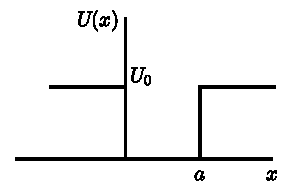
\includegraphics[width=4.5cm]{fig1.pdf}\\
{\small 图 1}
\end{center}

对 $E<U_0$ 而言，(22.2) 式在无穷远处为零的解为
\begin{equation}
  \psi=\text{常数}\times\mathrm{e}^{\mp\kappa x},
  \qquad\text{其中}\ \kappa=\frac{1}{\hbar}\sqrt{2m\left(U_0-E\right)}
\end{equation}
（指数上的 $-$ 号和 $+$ 号是分别对 $x>a$ 和 $x<0$ 两个区域而言的）.$E<U(x)$ 区域内发现粒子的概率 $|\psi|^2$ 作指数式递减.势阱边上的 $\psi$ 和 $\psi'$ 的连续性条件，为方便计，可用 $\psi$ 及其对数导数 $\psi'/\psi$ 的连续性条件来代替.计算 (22.3) 式，可得下列形式的边界条件：
\begin{equation}
  |\psi'|/\psi=\mp\kappa.
\end{equation}
我们不在这里讨论势阱深度 $U_0$ 为任意值时的能级问题（见习题 2），下面只对无限深势壁（$U_0\to\infty$）这一极限情形作出详细分析.

当 $U_0=\infty$ 时，§18中已经指出，粒子只能在 $x=0$ 和 $x=a$ 两点之间运动，这两个端点处的边界条件为
\begin{equation}
  \psi=0.
\end{equation}
[很易证明上式也可以由一般条件 (22.4) 式得出.因为 $U_0\to\infty$ 时同时有 $\kappa\to\infty$，从而有 $\psi'/\psi\to\infty$；由于 $\psi'$ 不能等于无穷大，故 $\psi=0$].势阱之内的 (22.1) 式具有以下形状的解：
\begin{equation}
  \psi=c\sin\left(kx+\delta\right),
  \qquad\text{其中}\ k=\frac{\sqrt{2mE}}{\hbar}.
\end{equation}
由 $x=0$ 时 $\psi=0$ 的条件，得 $\delta=0$，再按同一条件，在 $x=a$ 处给出 $\sin ka=0$，故 $ka=n\pi$（$n$ 为一正整数\footnote{$n=0$ 时将有 $\psi$ 恒等于零.}，从 1 开始）或
\begin{equation}
  E_n=\frac{\pi^2\hbar^2}{2ma^2}n^2,
  \qquad n=1,2,3,\cdots
\end{equation}
这个式子确定了势阱中一个粒子的各种能级.归一化的定态波函数为
\begin{equation}
  \psi_n=\sqrt{\frac{2}{a}}\sin\left(\pi nx/a\right).
\end{equation}
根据以上的结果我们可以直接写出一个粒子在直角“势箱”中的各种能级，该粒子在这个“势箱”中作三维运动，其势能当 $0<x<a$，$0<y<b$，$0<z<c$ 时为 $U=0$，在这个区域以外为 $U=\infty$.实际上，这种能级等于下列和量：
\begin{equation}
  E_{n_1 n_2 n_3}=\frac{\pi^2\hbar^2}{2m}
  \left(\frac{n_1^2}{a^2}+\frac{n_2^2}{b^2}+\frac{n_3^2}{c^2}\right),
  \qquad\left(n_1,n_2,n_3=1,2,3,\cdots\right),
\end{equation}
相应的波函数等于下列乘积：
\begin{equation}
  \psi_{n_1 n_2 n_3}=\sqrt{\frac{8}{abc}}\,
  \sin\frac{\pi n_1}{a}x\cdot\sin\frac{\pi n_2}{b}y\cdot\sin\frac{\pi n_3}{c}z.
\end{equation}
由 (22.7) 或 (22.9) 式可知，基态能量 $E_0$ 的数量级约为 $\hbar^2/ml^2$，$l$ 为粒子运动区域的线性尺度.这个结果和不确定度关系式相一致：当坐标不确定度约为 $l$ 时，动量的不确定度因而动量本身的数量级约为 $\hbar/l$；相应的能量均为 $\dfrac{1}{m}\left(\hbar/l\right)^2$.

\begin{xiti}

\noindent{\heiti 习题 1}\quad 在无限深的方势阱中，求一基态粒子的各种动量值的概率分布.

解：(22.8) 式的 $\psi_1$ 函数按动量本征函数展开后的展开系数 $a(p)$ 为
\begin{equation*}
  a(p)=\int\psi_p^*\psi_1\,\mathrm{d}x
  =\sqrt{\frac{2}{a}}\int_0^a\sin\left(\frac{\pi}{a}x\right)
  \mathrm{e}^{-(\mathrm{i}/\hbar)px}\,\mathrm{d}x.
\end{equation*}
做出积分后，再求其模量平方，即得下列概率分布：
\begin{equation*}
  |a(p)|^2\,\frac{\mathrm{d}p}{2\pi\hbar}
  =\frac{4\pi\hbar^3 a}{\left(p^2a^2-\pi^2\hbar^2\right)^2}
  \cos^2\frac{pa}{2\hbar}\,\mathrm{d}p
\end{equation*}

\noindent{\heiti 习题 2}\quad 求图 2 中势阱的能级.

解：我们考虑 $E<U_1$ 的离散谱.$x<0$ 区域内的波函数为
\begin{equation*}
  \psi=c_1\,\mathrm{e}^{\kappa_1 x},
  \qquad\text{其中}\ \kappa_1=\frac{1}{\hbar}\sqrt{2m\left(U_1-E\right)},
\end{equation*}
$x>a$ 区域内有
\begin{equation*}
  \psi=c_2\,\mathrm{e}^{-\kappa_2 x},
  \qquad\text{其中}\ \kappa_2=\frac{1}{\hbar}\sqrt{2m\left(U_2-E\right)}.
\end{equation*}

\begin{center}
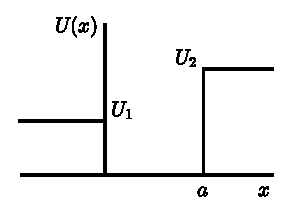
\includegraphics[width=5cm]{fig2.pdf}\\
{\small 图 2}
\end{center}

势阱内（$0<x<a$）的 $\psi$ 可取下列形式：
\begin{equation*}
  \psi=c\sin\left(kx+\delta\right),
  \qquad\text{其中}\ k=\frac{\sqrt{2mE}}{\hbar}.
\end{equation*}
根据势阱边上 $\psi'/\psi$ 的连续性条件，得
\begin{equation*}
  k\cot\delta=\kappa_1=\sqrt{\frac{2m}{\hbar^2}U_1-k^2},
  \qquad
  k\cot\left(ak+\delta\right)=-\kappa_2=-\sqrt{\frac{2m}{\hbar^2}U_2-k^2},
\end{equation*}
或
\begin{equation*}
  \sin\delta=\frac{k\hbar}{\sqrt{2mU_1}},
  \qquad
  \sin\left(ka+\delta\right)=-\frac{k\hbar}{\sqrt{2mU_2}}.
\end{equation*}
消去 $\delta$ 后，得下列超越方程：
\begin{equation*}
  ka=n\pi-\arcsin\frac{k\hbar}{\sqrt{2mU_1}}
  -\arcsin\frac{k\hbar}{\sqrt{2mU_2}}
\end{equation*}
（其中 $n=1,2,3,\cdots$，反正弦函数所取之值介于 0 到 $\dfrac{1}{2}\pi$ 之间），上式之根确定了能级 $E=k^2\hbar^2/2m$.对每一个 $n$ 一般来讲只有一个根；$n$ 值按能级的递增次序编号.

由于反正弦函数的宗量不能超过 1，$k$ 值显然只能介于 0 到 $\sqrt{2mU_1}/\hbar$ 之间.(1) 式的左边随 $k$ 单调地增大，该式的右边却随 $k$ 单调地减小.因此 (1) 式有根的必要条件为 $k=\sqrt{2mU_1}/\hbar$ 时，式右应该小于式左.特别是，由 $n=1$ 所得的下列不等式
\begin{equation*}
  a\,\frac{\sqrt{2mU_1}}{\hbar}\geqslant\frac{\pi}{2}
  -\arcsin\sqrt{\frac{U_1}{U_2}},
\end{equation*}
给出了阱中至少存在一个能级的条件.由此可见，给定了不相等的 $U_1$ 和 $U_2$ 后，总可以找到一个很窄的阱宽 $a$，使得该阱中不能存在离散能级.对 $U_1=U_2$ 而言，条件 (2) 总能得到满足.

$U_1=U_2\equiv U_0$（一个对称势阱）时，(1) 式可化成
\begin{equation*}
  \arcsin\frac{\hbar k}{\sqrt{2mU_0}}=\frac{1}{2}\left(n\pi-ka\right).
\end{equation*}
引进变量 $\xi=\dfrac{1}{2}ka$，当 $n$ 为奇数时，得下列方程：
\begin{equation*}
  \cos\xi=\pm\gamma\xi,
  \qquad\text{其中}\ \gamma=\frac{\hbar}{a}\sqrt{\frac{2}{mU_0}},
\end{equation*}
上式应取 $\tan\xi>0$ 的根.当 $n$ 为偶数时，可得
\begin{equation*}
  \sin\xi=\pm\gamma\xi
\end{equation*}
我们应取 $\tan\xi<0$ 的根.这两个方程式的根确定了 $E=2\xi^2\hbar^2/ma^2$ 能级，$\gamma\neq 0$ 时能级的总数为有限.

特别是对于 $U_0\ll\hbar^2/ma^2$ 的浅势阱，我们有 $\gamma\gg 1$，(5) 式根本无解.(4) 式有一个根（式右取 $+$ 号），等于 $\xi\approx\dfrac{1}{\gamma}\left(1-\dfrac{1}{2\gamma^2}\right)$.因此，阱中只包含有一个能级
\begin{equation*}
  E_0\approx U_0-\frac{ma^2}{2\hbar^2}U_0^2,
\end{equation*}
处于阱“口”附近.

\noindent{\heiti 习题 3}\quad 粒子在一直角“势箱”中运动，求箱壁所受的压强.

解：作用于垂直于 $x$ 轴的箱壁上的力，等于 $-\partial H/\partial a$（粒子的哈密顿函数对沿 $x$ 轴的箱长的微商）的平均值；此力除以该壁面积 $bc$ 后即得压强.根据 (11.16) 式，欲求的平均值可从 (22.9) 式能量本征值的微商得到.结果压强为
\begin{equation*}
  p^{(x)}=\frac{\pi^2\hbar^2}{ma^3bc}\,n_1^2.
\end{equation*}

\end{xiti}

\section{线性振子}

我们来考虑一个作一维小振动的粒子（称为一个线性振子）.该粒子的势能为 $m\omega^2x^2/2$，其中的 $\omega$ 为经典力学中的固有振动（圆）频率.该振子的哈密顿量因而是
\begin{equation}
  \hat{H}=\frac{\hat{p}^2}{2m}+\frac{m\omega^2x^2}{2}.
\end{equation}
由于 $x\to\pm\infty$ 时势能为无穷大，该粒子只能作有限运动，其能谱完全是离散的.

我们试用矩阵方法\footnote{这是在薛定谔波动方程未发现前由海森伯于 1925 年所作的.}求解该振子的能级.我们从 (19.3) 形式的“运动方程”出发；在目前情形下，由该式得
\begin{equation}
  \hat{\ddot{x}}+\omega^2\hat{x}=0.
\end{equation}
此式的矩阵形式为
\begin{equation*}
  \left(\ddot{x}\right)_{mn}+\omega^2 x_{mn}=0.
\end{equation*}
根据 (11.8) 式，加速度的矩阵元
$\left(\ddot{x}\right)_{mn}=\mathrm{i}\omega_{mn}\left(\dot{x}\right)_{mn}=-\omega_{mn}^2 x_{mn}$.因此，得
\begin{equation*}
  \left(\omega_{mn}^2-\omega^2\right)x_{mn}=0.
\end{equation*}
由此可见，矩阵元 $x_{mn}$ 除了 $\omega_{mn}=\pm\omega$ 以外显然都等于零.我们把所有的定态加以编号，使得 $n\to n\pm 1$ 的跃迁频率为 $\pm\omega$，即 $\omega_{n,n\mp 1}=\pm\omega$.此时不等于零的矩阵元只有 $x_{n,n\pm 1}$.

现在假定所有的波函数 $\psi_n$ 都取实函数.由于 $x$ 为实量，从而所有的矩阵元 $x_{mn}$ 都是实数.厄米条件 (11.10) 式表明，这样的 $x_{mn}$ 矩阵是一个对称矩阵：即满足 $x_{mn}=x_{nm}$.

为了算出不等于零的矩阵元，我们利用下列对易关系：
\begin{equation*}
  \hat{\dot{x}}\hat{x}-\hat{x}\hat{\dot{x}}=-\mathrm{i}\frac{\hbar}{m},
\end{equation*}
把它写成矩阵形式：
\begin{equation*}
  \left(\dot{x}\,x\right)_{mn}-\left(x\dot{x}\right)_{mn}
  =-\frac{\mathrm{i}\hbar}{m}\delta_{mn}.
\end{equation*}
利用矩阵乘法法则 (11.12)，当 $m=n$ 时，上式为
\begin{equation*}
  \mathrm{i}\sum_l\left(\omega_{nl}x_{nl}x_{ln}
  -x_{nl}\omega_{ln}x_{ln}\right)
  =2\mathrm{i}\sum_l\omega_{nl}x_{nl}^2
  =-\mathrm{i}\frac{\hbar}{m}.
\end{equation*}
这个求和式中，只有 $l=n\pm 1$ 的项不等于零，故得
\begin{equation}
  \left(x_{n+1,n}\right)^2-\left(x_{n,n-1}\right)^2
  =\frac{\hbar}{2m\omega}.
\end{equation}
上式表明，$\left(x_{n+1,n}\right)^2$ 诸量组成一个算术级数，因为它们只能是正的，这组量没有上限但有下限.由于我们只编定了各态的相对位置，还没有确定编号 $n$ 的绝对值，我们可以任选一个 $n$ 值对应于振子的第一态（基态）.现在取这个 $n$ 值等于零.因此 $x_{0,-1}$ 现在必须看作恒等于零，依次应用 $n=0,1,\cdots$ 的 (23.3) 式，可导出下列结果：
\begin{equation*}
  \left(x_{n,n-1}\right)^2=\frac{n\hbar}{2m\omega}.
\end{equation*}
因此最后得下列不等于零的坐标矩阵元\footnote{我们选择未确定的相位 $\alpha_n$（见 §11 第三个脚注），使得 (23.4) 式的所有矩阵元在平方根前均取正号.这样的选择总是可能的，因为这个矩阵中只有相邻两态间的跃迁矩阵元才不等于零.}：
\begin{equation}
  x_{n,n-1}=x_{n-1,n}=\sqrt{\frac{n\hbar}{2m\omega}}.
\end{equation}
算符 $\hat{H}$ 的矩阵是对角的，并且矩阵元 $H_{nn}$ 就是欲求的振子能量本征值 $E_n$.它的计算方法如下：
\begin{equation*}
\begin{aligned}
  H_{nn}=E_n
  &=\frac{m}{2}\left[\left(\dot{x}^2\right)_{nn}
  +\omega^2\left(x^2\right)_{nn}\right]=\\
  &=\frac{m}{2}\left[\sum_l\mathrm{i}\omega_{nl}x_{nl}\,\mathrm{i}\omega_{ln}x_{ln}
  +\omega^2\sum_l x_{nl}x_{ln}\right]=\\
  &=\frac{m}{2}\sum_l\left(\omega^2+\omega_{nl}^2\right)x_{ln}^2.
\end{aligned}
\end{equation*}
对 $l$ 求和时，只有 $l=n\pm 1$ 的两项不等于零；用 (23.4) 式代入，得
\begin{equation}
  E_n=\left(n+\frac{1}{2}\right)\hbar\omega,
  \qquad n=0,1,2,\cdots
\end{equation}
由此可见，振子的各个能级是以等间隔 $\hbar\omega$ 依次排列的.基态（$n=0$）能量为 $\dfrac{1}{2}\hbar\omega$；注意，它并不等于零.

式 (23.5) 的结果也可以从振子的薛定谔方程中直接解出来.这个方程的形式为
\begin{equation}
  \frac{\mathrm{d}^2\psi}{\mathrm{d}x^2}
  +\frac{2m}{\hbar^2}
  \left(E-\frac{m}{2}\omega^2x^2\right)\psi=0.
\end{equation}
为方便计，最好将坐标变量 $x$ 换成以下所示的量纲为 1 的变量 $\xi$：
\begin{equation}
  \xi=\sqrt{\frac{m\omega}{\hbar}}\,x.
\end{equation}
则方程式成为
\begin{equation}
  \psi''+\left[\left(2E/\hbar\omega\right)-\xi^2\right]\psi=0.
\end{equation}
式中的撇号现在代表对 $\xi$ 求微商.

当 $\xi$ 很大时，$2E/\hbar\omega$ 和 $\xi^2$ 相比可以略去不计；方程式 $\psi''=\xi^2\psi$ 具有渐近积分 $\psi=\mathrm{e}^{\pm\frac{1}{2}\xi^2}$（对这个函数求微商后，略去数量级较小的项，可得 $\psi''=\xi^2\psi$）.由于 $\xi\to\pm\infty$ 时波函数 $\psi$ 必须保持有限，指数上的符号只能取负号.因此，我们自然用下式代入 (23.8) 式：
\begin{equation}
  \psi=\mathrm{e}^{-\frac{1}{2}\xi^2}\chi(\xi).
\end{equation}
结果得函数 $\chi(\xi)$ 的一个方程式
\begin{equation}
  \chi''-2\xi\chi'+2n\chi=0
\end{equation}
[式中的 $2n=\left(2E/\hbar\omega\right)-1$；我们已知 $E>0$，故有 $n>-\dfrac{1}{2}$]，式中的函数 $\chi$ 对 $\xi$ 的所有有限值而言必须保持有限，且当 $\xi\to\pm\infty$ 时，不能比 $\xi$ 的任一有限次幂更快地趋向无穷大（以便使函数 $\psi$ 能趋于零）.

只有当 $n$ 等于正整数（及零）时，(23.10) 式才能有这样的解（见数学附录§a）；它所给出的能量本征值就是我们早已知道的 (23.5) 式.(23.10) 式中，当 $n$ 等于各种正整数值时，它的相应解为 $\chi=$ 常数 $\times\,H_n(\xi)$，其中的 $H_n(\xi)$ 称为厄米多项式，它们是 $\xi$ 的 $n$ 次多项式，其定义为
\begin{equation}
  H_n(\xi)=\left(-1\right)^n
  \mathrm{e}^{\xi^2}\mathrm{d}^n\left(\mathrm{e}^{-\xi^2}\right)/\mathrm{d}\xi^n.
\end{equation}
求出 $\psi_n$ 中的常数，使 $\psi_n$ 满足归一化条件
\begin{equation*}
  \int_{-\infty}^{\infty}\psi_n^2(x)\,\mathrm{d}x=1,
\end{equation*}
结果得[见附录 (a.7) 式]
\begin{equation}
  \psi_n(x)=\left(\frac{m\omega}{\pi\hbar}\right)^{\frac{1}{4}}
  \frac{1}{\sqrt{2^n n!}}\,
  \mathrm{e}^{-\frac{m\omega}{2\hbar}x^2}
  H_n\left(x\sqrt{\frac{m\omega}{\hbar}}\right).
\end{equation}
故基态波函数为
\begin{equation}
  \psi_0(x)=\left(\frac{m\omega}{\hbar\pi}\right)^{\frac{1}{4}}
  \mathrm{e}^{-\frac{m\omega}{2\hbar}x^2}.
\end{equation}
理所当然，这个函数对有限的 $x$ 值而言并无零点.

计算积分式 $\int_{-\infty}^{\infty}\psi_n\psi_m\xi\,\mathrm{d}\xi$，可给出坐标的矩阵元；其结果当然也和 (23.4) 式给出的值相同.

最后，我们来看一下如何用矩阵方法求出 $\psi_n$ 波函数.我们注意到，$\hat{\dot{x}}\pm\mathrm{i}\omega\hat{x}$ 算符的矩阵中不等于零的矩阵元只有
\begin{equation}
  \left(\dot{x}-\mathrm{i}\omega x\right)_{n-1,n}
  =-\left(\dot{x}+\mathrm{i}\omega x\right)_{n,n-1}
  =-\mathrm{i}\sqrt{\frac{2\omega\hbar n}{m}}.
\end{equation}
应用 (11.11) 的普遍公式，并且考虑到 $\psi_{-1}\equiv 0$，可得下列结论：
\begin{equation*}
  \left(\hat{\dot{x}}-\mathrm{i}\omega x\right)\psi_0=0.
\end{equation*}
把 $\hat{\dot{x}}=-\mathrm{i}\dfrac{\hbar}{m}\dfrac{\mathrm{d}}{\mathrm{d}x}$ 代入上式后得到以下方程式：
\begin{equation*}
  \frac{\mathrm{d}\psi_0}{\mathrm{d}x}
  =-\frac{m\omega}{\hbar}x\psi_0,
\end{equation*}
这式的归一化解就是 (23.13) 式.并由于
\begin{equation*}
  \left(\dot{x}+\mathrm{i}\omega x\right)\psi_{n-1}
  =\left(\dot{x}+\mathrm{i}\omega x\right)_{n,n-1}\psi_n
  =\mathrm{i}\sqrt{\frac{2\omega\hbar n}{m}}\,\psi_n,
\end{equation*}
我们得循环式
\begin{equation*}
\begin{aligned}
  \psi_n
  &=\sqrt{\frac{m}{2\omega\hbar n}}
  \left(-\frac{\hbar}{m}\frac{\mathrm{d}}{\mathrm{d}x}+\omega x\right)\psi_{n-1}
  =\\
  &=\frac{1}{\sqrt{2n}}\left(-\frac{\mathrm{d}}{\mathrm{d}\xi}+\xi\right)\psi_{n-1}
  =-\frac{1}{\sqrt{2n}}\,
  \mathrm{e}^{\frac{1}{2}\xi^2}\frac{\mathrm{d}}{\mathrm{d}\xi}
  \left(\mathrm{e}^{-\frac{1}{2}\xi^2}\psi_{n-1}\right),
\end{aligned}
\end{equation*}
上式对 (23.13) 式的 $\psi_0$ 函数连用 $n$ 次，即得 (23.12) 式中的归一化波函数 $\psi_n$.

\begin{xiti}

\noindent{\heiti 习题 1}\quad 试求振子的各种动量值的概率分布.

解：在振子情形下，不采用把定态波函数展开成动量本征函数组的方法，而直接从动量表象中的薛定谔方程出发比较来得简单.把 (15.12) 式的坐标算符
$\hat{x}=\mathrm{i}\hbar\left(\mathrm{d}/\mathrm{d}p\right)$
代入 (23.1) 式，可得“$p$ 表象”中的哈密顿量：
\begin{equation*}
  \hat{H}=\frac{p^2}{2m}
  -\frac{m\omega^2\hbar^2}{2}\frac{\mathrm{d}^2}{\mathrm{d}p^2}
\end{equation*}
$p$ 表象中的波函数 $a(p)$ 所满足的薛定谔方程 $\hat{H}a(p)=Ea(p)$ 为
\begin{equation*}
  \frac{\mathrm{d}^2 a(p)}{\mathrm{d}p^2}
  +\frac{2}{m\omega^2\hbar^2}
  \left(E-\frac{p^2}{2m}\right)a(p)=0.
\end{equation*}
这个方程正好和 (23.6) 式具有相同的形式，故其解可以参照 (23.12) 式立即写出来，由此得出欲求的概率分布为
\begin{equation*}
  |a_n(p)|^2\,\frac{\mathrm{d}p}{2\pi\hbar}
  =\frac{1}{2^n n!\,\sqrt{\pi m\omega\hbar}}\,
  \mathrm{e}^{-p^2/(m\omega\hbar)}
  H_n^2\left(\frac{p}{\sqrt{m\omega\hbar}}\right)\mathrm{d}p
\end{equation*}

\noindent{\heiti 习题 2}\quad 试用不确定度关系式 (16.7)，求振子能量可能值的下限.

解：由于 $\overline{x^2}=\bar{x}^2+\left(\delta x\right)^2$，
$\overline{p^2}=\bar{p}^2+\left(\delta p\right)^2$，
(16.7) 给出振子能量平均值
\begin{equation*}
  \overline{E}=\frac{m\omega^2}{2}\overline{x^2}
  +\frac{\overline{p^2}}{2m}
  \geqslant\frac{m\omega^2}{2}\left(\delta x\right)^2
  +\frac{1}{2m}\left(\delta p\right)^2
  \geqslant\frac{m\omega^2\hbar^2}{8\left(\delta p\right)^2}
  +\frac{1}{2m}\left(\delta p\right)^2,
\end{equation*}
求出上式的极小值（看作 $\delta p$ 的函数），即得能量平均值的下限，故对能量的所有可能值，有
\begin{equation*}
  E\geqslant\frac{1}{2}\hbar\omega.
\end{equation*}

\noindent{\heiti 习题 3}\quad 求线性振子的状态波函数，这些态的测不准关系具有极小值，即波包中的坐标和动量标准偏差具有关系式
$\delta p\,\delta x=\dfrac{1}{2}\hbar$（E.~薛定谔，1926）\footnote{这些态称为相干态.}.

解：所求的波函数应具下列形式：
\begin{equation*}
  \varPsi(x,t)=\frac{1}{\left(2\pi\right)^{1/4}\left(\delta x\right)^{1/2}}
  \exp\left\{\frac{\mathrm{i}\bar{p}x}{\hbar}
  -\frac{\left(x-\bar{x}\right)^2}{4\left(\delta x\right)^2}
  -\mathrm{i}\phi(t)\right\},
\end{equation*}
式中任一时刻的坐标依赖关系与 (16.8) 式一致，$\bar{x}=\bar{x}(t)$ 和
$\bar{p}=\bar{p}(t)=m\dot{\bar{x}}(t)$ 是坐标和动量的平均值；根据 (19.3) 式，对线性振子来讲 $U=\dfrac{1}{2}m\omega^2x^2$，我们有 $\hat{\dot{p}}=-m\omega^2 x$，故其平均值 $\dot{\bar{p}}=-m\omega^2\bar{x}$，或
\begin{equation*}
  \ddot{\bar{x}}+\omega^2\bar{x}=0.
\end{equation*}
亦即 $\bar{x}(t)$ 函数满足经典运动方程.(1) 式中的常数因子应由以下的归一化条件确定：
\begin{equation*}
  \int_{-\infty}^{\infty}|\varPsi|^2\,\mathrm{d}x=1;
\end{equation*}
除了这个因子外，$\varPsi$ 中还可含有一个相位因子，其相位 $\phi(t)$ 与时间有关.为求未知常数 $\delta x$ 和未知函数 $\phi(t)$，可把 (1) 式代入下列波动方程
\begin{equation*}
  -\frac{\hbar^2}{2m}\frac{\partial^2\varPsi}{\partial x^2}
  +\frac{1}{2}m\omega^2 x^2\varPsi
  =\mathrm{i}\hbar\frac{\partial\varPsi}{\partial t}.
\end{equation*}
代入后利用 (2) 式，得
\begin{equation*}
  \left(\frac{1}{2}x^2-x\bar{x}\right)
  \left(\frac{m^2\omega^2}{\hbar^2}
  -\frac{1}{4\left(\delta x\right)^4}\right)
  +\left[\frac{m^2\dot{\bar{x}}^2}{2\hbar^2}
  -\frac{\bar{x}^2}{8\left(\delta x\right)^4}
  +\frac{1}{4\left(\delta x\right)^2}
  -\frac{m}{\hbar}\dot{\phi}(t)\right]=0,
\end{equation*}
从而得 $\left(\delta x\right)^2=\hbar/2m\omega$ 及
\begin{equation*}
  \dot{\phi}=\frac{m}{2\hbar}
  \left(\dot{\bar{x}}^2-\omega^2\bar{x}^2\right)+\frac{1}{2}\omega,
\end{equation*}
\begin{equation*}
  \phi=\frac{1}{2\hbar}\bar{p}\bar{x}+\frac{1}{2}\omega t.
\end{equation*}
因此最后得
\begin{equation*}
  \varPsi(x,t)=\left(\frac{m\omega}{\pi\hbar}\right)^{1/4}
  \exp\left\{\frac{\mathrm{i}\bar{p}x}{\hbar}
  -\frac{m\omega\left(x-\bar{x}\right)^2}{2\hbar}\right\}
  \cdot\exp\left\{-\frac{1}{2}\mathrm{i}\omega t
  -\frac{\mathrm{i}\bar{p}\bar{x}}{2\hbar}\right\}
\end{equation*}
当 $\bar{x}=0$ 和 $\bar{p}=0$ 时，上式变成 $\psi_0(x)\,\mathrm{e}^{-\mathrm{i}\omega t/2}$，即振子的基态波函数.

相干态中振子的平均能量为
\begin{equation*}
\begin{aligned}
  \overline{E}
  &=\frac{\overline{p^2}}{2m}
  +\frac{1}{2}m\omega^2\overline{x^2}=\\
  &=\frac{\bar{p}^2}{2m}
  +\frac{1}{2}m\omega^2\bar{x}^2+\frac{1}{2}\hbar\omega
  =\hbar\omega\left(\bar{n}+\frac{1}{2}\right)
\end{aligned}
\end{equation*}
$n$ 为该态中量子 $\hbar\omega$ 的平均“数”.由此可知，相干态完全是由满足经典方程 (2) 的 $\bar{x}(t)$ 函数确定的.这个函数的一般形式可用下式给出：
\begin{equation*}
  \frac{m\omega\bar{x}+\mathrm{i}\bar{p}}{\sqrt{2m\hbar\omega}}
  =a\,\mathrm{e}^{-\mathrm{i}\omega t},
  \qquad|a|^2=\bar{n}
\end{equation*}
函数 (3) 可按振子的定态波函数展开：
\begin{equation*}
  \psi=\sum_{n=0}^{\infty}a_n\psi_n,
\end{equation*}
\begin{equation*}
  \varPsi_n(x,t)=\psi_n(x)
  \exp\left\{-\mathrm{i}\left(n+\frac{1}{2}\right)\omega t\right\},
\end{equation*}
式中的展开系数为（参考§41，题 1）
\begin{equation*}
  a_n=\int_{-\infty}^{\infty}\psi_n^*\psi\,\mathrm{d}x.
\end{equation*}
从而得振子处于第 $n$ 个定态的概率
\begin{equation*}
  w_n=|a_n|^2=\mathrm{e}^{-\bar{n}}\frac{\bar{n}^n}{n!}.
\end{equation*}
这是泊松分布.

\noindent{\heiti 习题 4}\quad 一个粒子在下列势场中运动（图 3）
\begin{equation*}
  U(x)=A\left(\mathrm{e}^{-2\alpha x}-2\,\mathrm{e}^{-\alpha x}\right)
\end{equation*}
试求其能级（P.M.~Morse）.

\begin{center}
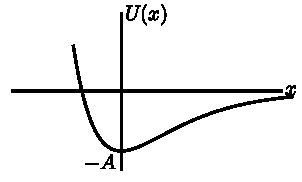
\includegraphics[width=5.5cm]{fig3.pdf}\\
{\small 图 3}
\end{center}

解：正能量本征值呈连续谱（且其能级无简并），而负能量本征值呈离散谱.

薛定谔方程为
\begin{equation*}
  \frac{\mathrm{d}^2\psi}{\mathrm{d}x^2}
  +\frac{2m}{\hbar^2}
  \left(E-A\,\mathrm{e}^{-2\alpha x}
  +2A\,\mathrm{e}^{-\alpha x}\right)\psi=0,
\end{equation*}
引进一个新变量
\begin{equation*}
  \xi=\frac{2\sqrt{2mA}}{\alpha\hbar}\,\mathrm{e}^{-\alpha x}
\end{equation*}
（其值从 0 到 $+\infty$），并令（我们考虑离散谱，故 $E<0$）
\begin{equation*}
  s=\frac{\sqrt{-2mE}}{\alpha\hbar},
  \qquad
  n=\frac{\sqrt{2mA}}{\alpha\hbar}-\left(s+\frac{1}{2}\right),
\end{equation*}
则薛定谔方程呈以下形式：
\begin{equation*}
  \psi''+\frac{1}{\xi}\psi'
  +\left(-\frac{1}{4}
  +\frac{n+s+\frac{1}{2}}{\xi}
  -\frac{s^2}{\xi^2}\right)\psi=0.
\end{equation*}
当 $\xi\to\infty$ 时，函数 $\psi$ 的渐近行为和 $\mathrm{e}^{\pm\frac{1}{2}\xi}$ 一样，而当 $\xi\to 0$ 时，$\psi$ 和 $\xi^{\pm s}$ 成正比.考虑到波函数的有限性，我们所选的解当 $\xi\to\infty$ 时必须像 $\mathrm{e}^{-\frac{1}{2}\xi}$ 那样，而当 $\xi\to 0$ 时必须像 $\xi^s$ 那样.因而作下列变换：
\begin{equation*}
  \varPsi=\mathrm{e}^{-\xi/2}\xi^s w(\xi)
\end{equation*}
可得下列 $w$ 的方程式
\begin{equation*}
  \xi w''+\left(2s+1-\xi\right)w'+nw=0,
\end{equation*}
求解 $w$ 时，要求 $w$ 当 $\xi\to 0$ 时为有限，$\xi\to\infty$ 时 $w$ 不能比 $\xi$ 的任一有限次幂更快地趋向无穷大.(2) 式是一个合流超几何函数的方程式（见数学附录§d）；
\begin{equation*}
  w=F\left(-n,\,2s+1,\,\xi\right).
\end{equation*}
$n$ 为非负整数时即得满足所需条件的解（此时 $F$ 函数变成一个多项式）.按定义 (1)，由此得出的能级值为
\begin{equation*}
  -E_n=A\left[1-\frac{\alpha\hbar}{\sqrt{2mA}}
  \left(n+\frac{1}{2}\right)\right]^2,
\end{equation*}
其中的 $n$ 为正整数，$n$ 的数值可以从零开始一直到满足
$\dfrac{1}{\alpha\hbar}\sqrt{2mA}>n+\dfrac{1}{2}$
的最大整数值为止（因按定义参量 $s$ 是正的），因此离散谱中只包含有限多个能级.如果 $\sqrt{2mA}/\alpha\hbar<\dfrac{1}{2}$，离散谱就根本不存在.

\noindent{\heiti 习题 5}\quad 上题中 $U=-U_0/\cosh^2\alpha x$（见图 4）.

\begin{center}
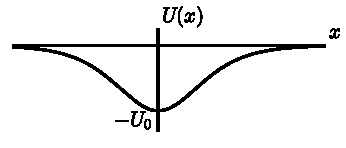
\includegraphics[width=6cm]{fig4.pdf}\\
{\small 图 4}
\end{center}

解：正能量本征值呈连续谱，负能量本征值呈离散谱；我们只考虑后一种情况.薛定谔方程为
\begin{equation*}
  \frac{\mathrm{d}^2\psi}{\mathrm{d}x^2}
  +\frac{2m}{\hbar^2}
  \left(E+\frac{U_0}{\cosh^2\alpha x}\right)\psi=0.
\end{equation*}
把变量换成 $\xi=\tanh\alpha x$，并令
\begin{equation*}
  \varepsilon=\frac{\sqrt{-2mE}}{\alpha\hbar},
  \qquad
  \frac{2mU_0}{\alpha^2\hbar^2}=s\left(s+1\right),
  \qquad
  s=\frac{1}{2}\left(-1+\sqrt{1+\frac{8mU_0}{\alpha^2\hbar^2}}\right),
\end{equation*}
可得
\begin{equation*}
  \frac{\mathrm{d}}{\mathrm{d}\xi}
  \left[\left(1-\xi^2\right)\frac{\mathrm{d}\psi}{\mathrm{d}\xi}\right]
  +\left[s\left(s+1\right)
  -\frac{\varepsilon^2}{1-\xi^2}\right]\psi=0.
\end{equation*}
这是缔合勒让德函数的方程.如令
\begin{equation*}
  \psi=\left(1-\xi^2\right)^{\varepsilon/2}w(\xi),
\end{equation*}
并把变量暂时改成 $u=\dfrac{1}{2}\left(1-\xi\right)$，则上式可变为下列超几何方程：
\begin{equation*}
  u\left(1-u\right)w''
  +\left(\varepsilon+1\right)\left(1-2u\right)w'
  -\left(\varepsilon-s\right)\left(\varepsilon+s+1\right)w=0.
\end{equation*}
$\xi=1$（即 $x=\infty$）时取有限值的解为
\begin{equation*}
  \psi=\left(1-\xi^2\right)^{\varepsilon/2}
  F\left[\varepsilon-s,\,\varepsilon+s+1,\,
  \varepsilon+1,\,\left(1-\xi\right)/2\right].
\end{equation*}
为了使 $\psi$ 当 $\xi=-1$（即 $x=-\infty$）时保持有限，必须有 $\varepsilon-s=-n$，而 $n=0,1,2,\cdots$；此时 $F$ 是一个 $n$ 次多项式，$\xi=-1$ 时 $F$ 为有限.

因此能级由条件 $s-\varepsilon=n$ 所确定，得出
\begin{equation*}
  E_n=-\frac{\hbar^2\alpha^2}{8m}
  \left[-\left(1+2n\right)
  +\sqrt{1+\frac{8mU_0}{\alpha^2\hbar^2}}\right]^2.
\end{equation*}
根据 $\varepsilon>0$ 即 $n<s$ 的条件可知，能级总数为有限.

\end{xiti}

\section{均匀场中的运动}

考虑一个粒子在一均匀外场中运动.取外场方向为 $x$ 轴方向，令 $F$ 为粒子在该场中所受的力；对强度为 $E$ 的电场而言，此力 $F=eE$，$e$ 为粒子的电荷.

均匀场中的粒子势能呈 $U=-Fx+$ 常数 的形式；选常数使得 $x=0$ 时 $U=0$，则有 $U=-Fx$.这个问题的薛定谔方程为
\begin{equation}
  \frac{\mathrm{d}^2\psi}{\mathrm{d}x^2}
  +\frac{2m}{\hbar^2}\left(E+Fx\right)\psi=0.
\end{equation}
由于 $x\to-\infty$ 时 $U$ 趋向 $+\infty$，$x\to+\infty$ 时 $U\to-\infty$，各能级显然组成连续谱，能量 $E$ 的值域占有从 $-\infty$ 直到 $+\infty$ 的整个区域.其中没有一个本征值是简并的，所对应的运动向 $x=-\infty$ 方向为有限，向 $x\to+\infty$ 方向为无限.

我们引入下列量纲为 1 的变量来代替原来的坐标变量 $x$：
\begin{equation}
  \xi=\left(x+\frac{E}{F}\right)
  \left(\frac{2mF}{\hbar^2}\right)^{1/3}.
\end{equation}
则 (24.1) 式呈以下形式：
\begin{equation}
  \psi''+\xi\psi=0.
\end{equation}
此式不含能量参量.因此，如能求出一个解满足有限性等必需条件，则立刻得到任意能量值的本征函数.

(24.3) 式中对所有 $x$ 都取有限值的解呈下列形式（见数学附录§b）：
\begin{equation}
  \psi(\xi)=A\,\varPhi(-\xi),
\end{equation}
其中
\begin{equation*}
  \varPhi(\xi)=\frac{1}{\sqrt{\pi}}
  \int_0^{+\infty}\cos\left(\frac{1}{3}u^3+u\xi\right)\mathrm{d}u
\end{equation*}
称为艾里函数，$A$ 为归一化因子，将在下面确定之.

当 $\xi\to-\infty$ 时，$\psi(\xi)$ 函数按指数规律趋于零.$\xi$ 为很大的负值时，$\psi(\xi)$ 的渐近式为[见 (b.4) 式]：
\begin{equation}
  \psi(\xi)\approx\frac{A}{2|\xi|^{1/4}}
  \exp\left[-\frac{2}{3}|\xi|^{3/2}\right].
\end{equation}
当 $\xi$ 为很大正值时，$\psi(\xi)$ 的渐近式为[见 (b.5) 式\footnote{顺便指出，渐近表式 (24.5) 和 (24.6) 对应于波函数在经典禁区和通区内的准经典表式（§47）.}]
\begin{equation}
  \psi(\xi)=A\xi^{-\frac{1}{4}}
  \sin\left(\frac{2}{3}\xi^{3/2}+\frac{1}{4}\pi\right).
\end{equation}
根据连续谱波函数的一般归一化法则 (5.4) 式，我们可以把 (24.4) 式化成一个函数，它归一化成能量的 $\delta$ 函数.即
\begin{equation}
  \int_{-\infty}^{\infty}\psi(\xi)\psi(\xi')\,\mathrm{d}x
  =\delta\left(E'-E\right).
\end{equation}
§21中曾经给出过一个简单方法，利用波函数的渐近式求出归一化系数.应用这个方法，我们首先把 (24.6) 式写成两个行波之和
\begin{equation*}
\begin{aligned}
  \psi(\xi)&\approx\frac{1}{2}A\xi^{-\frac{1}{4}}
  \exp\left(\mathrm{i}\left[\frac{2}{3}\xi^{3/2}-\frac{1}{4}\pi\right]\right)+\\
  &\qquad+\frac{1}{2}A\xi^{-\frac{1}{4}}
  \exp\left(-\mathrm{i}\left[\frac{2}{3}\xi^{3/2}-\frac{1}{4}\pi\right]\right).
\end{aligned}
\end{equation*}
由以上两项分别算出的概率流密度等于
\begin{equation*}
  v\left(\frac{A}{2\xi^{1/4}}\right)^2
  =\sqrt{\frac{2\left(E+Fx\right)}{m}}
  \left(\frac{A}{2\xi^{1/4}}\right)^2
  =A^2\,\frac{\left(2\hbar F\right)^{1/3}}{4m^{2/3}}.
\end{equation*}
令上式等于 $1/2\pi\hbar$，得到
\begin{equation}
  A=\frac{\left(2m\right)^{1/3}}
  {\pi^{1/2}F^{1/6}\hbar^{2/3}}.
\end{equation}

\begin{xiti}

\noindent{\heiti 习题}\quad 求处于均匀场中的一个粒子在动量表象中的波函数.

解：动量表象中的哈密顿算符为
\begin{equation*}
  \hat{H}=\frac{1}{2m}\,p^2-\mathrm{i}\hbar F\,\frac{\mathrm{d}}{\mathrm{d}p}
\end{equation*}
故波函数 $a(p)$ 所满足的薛定谔方程具有下列形状
\begin{equation*}
  -\mathrm{i}\hbar F\frac{\mathrm{d}a}{\mathrm{d}p}
  +\left(\frac{p^2}{2m}-E\right)a=0.
\end{equation*}
解出此式，即得欲求的波函数
\begin{equation*}
  a_E(p)=\frac{1}{\sqrt{2\pi\hbar F}}\,
  \exp\left[\frac{\mathrm{i}}{\hbar F}
  \left(Ep-\frac{p^3}{6m}\right)\right].
\end{equation*}
这种函数已按下列条件归一化：
\begin{equation*}
  \int_{-\infty}^{\infty}a_E^*(p)\,a_{E'}(p)\,\mathrm{d}p
  =\delta\left(E'-E\right).
\end{equation*}

\end{xiti}

\section{透射系数}

我们来考虑一个粒子，在图 5 所示的那类势场中运动：$U(x)$ 从某一固定极限值（$x\to-\infty$ 时的 $U=0$）开始，单调地增加到另一固定极限值（$x\to+\infty$ 时的 $U=U_0$）.根据经典力学，能量 $E<U_0$ 的一个粒子在这样的势场中自左向右运动时，碰到“势壁”以后会“反射”回来并开始沿相反的方向运动；但如 $E>U_0$，该粒子将沿原方向继续运动下去，只是会减速.量子力学中则会产生一种新的现象：即使 $E>U_0$，粒子仍有可能被势壁所“反射”.它的反射概率原则上可用下法算出.

\begin{center}
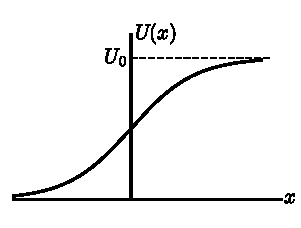
\includegraphics[width=5.5cm]{fig5.pdf}\\
{\small 图 5}
\end{center}

设粒子自左向右运动.当 $x$ 为很大正值时，波函数应该描述越过“壁顶”并沿 $x$ 轴的正方向运动的一个粒子，它的渐近式必然是
\begin{equation}
  \psi\approx A\,\mathrm{e}^{\mathrm{i}k_2x}
  \quad\left(x\to\infty\ \text{时}\right),
  \qquad\text{式中}\ k_2=\frac{1}{\hbar}\sqrt{2m\left(E-U_0\right)},
\end{equation}
$A$ 是一个常数.为了求出满足以上边界条件的薛定谔方程之解，我们来计算 $x\to-\infty$ 时的渐近式；这个渐近式等于自由运动方程中两个独立解的线性组合，具有下列形式
\begin{equation}
  \psi\approx\mathrm{e}^{\mathrm{i}k_1x}+B\,\mathrm{e}^{-\mathrm{i}k_1x}
  \quad\left(x\to-\infty\ \text{时}\right),
  \qquad
  k_1=\frac{1}{\hbar}\sqrt{2mE}.
\end{equation}
第一项相当于射向势壁的粒子（我们假定 $\psi$ 已经归一化成这样，使得该项的系数等于 1）；第二项代表由势壁反射回来的粒子.入射波的概率流密度为 $k_1$，而反射波为 $k_1|B|^2$，透射波为 $k_2|A|^2$.我们把粒子的透射系数 $D$ 定义成为透射波的概率流密度与入射波的概率流密度之比：
\begin{equation}
  D=\left(k_2/k_1\right)|A|^2.
\end{equation}
同理可以定义反射系数 $R$，它等于反射波与入射波的概率流密度之比.显然有 $R=1-D$，
\begin{equation}
  R=|B|^2=1-\left(k_2/k_1\right)|A|^2
\end{equation}
（$A$ 和 $B$ 自动满足此关系式）.

如果粒子自左向右运动而能量 $E<U_0$，则 $k_2$ 为纯虚数，$x\to+\infty$ 时波函数呈指数式衰减.反射流量就和入射流量相等，亦即粒子从势壁“全反射”.但须指出，在这种情形下，$E<U$ 区域内找到粒子的概率仍不等于零，但随 $x$ 的增大而很快地减小.

一般情形下，任意定态（能量 $E>U_0$）波函数的渐近式，不论是 $x\to-\infty$ 或 $x\to+\infty$，都可以写成沿 $x$ 轴的相反方向行进的两个平面波之和：
\begin{equation}
\begin{aligned}
  &x\to-\infty\ \text{时},\qquad
  \psi=A_1\mathrm{e}^{\mathrm{i}k_1x}+B_1\mathrm{e}^{-\mathrm{i}k_1x},\\
  &x\to+\infty\ \text{时},\qquad
  \psi=A_2\mathrm{e}^{\mathrm{i}k_2x}+B_2\mathrm{e}^{-\mathrm{i}k_2x}.
\end{aligned}
\end{equation}
由于以上两式都是线性微分方程的同一个解的渐近式，系数 $A_1,B_1$ 和 $A_2,B_2$ 之间存在着线性关系.设 $A_2=\alpha A_1+\beta B_1$，其中的 $\alpha$ 和 $\beta$ 是两个常数（一般讲来是复数），依赖于势场 $U(x)$ 的具体形状.如果考虑到薛定谔方程是实方程，我们还可以写出 $B_2$ 的相应关系式.这就是说，设 $\psi$ 为所给薛定谔方程之解，则其共轭复函数 $\psi^*$ 也是该方程之解.它的渐近形式为
\begin{equation*}
\begin{aligned}
  &x\to-\infty\ \text{时},\quad
  \psi^*=A_1^*\mathrm{e}^{-\mathrm{i}k_1x}+B_1^*\mathrm{e}^{\mathrm{i}k_1x},\\
  &x\to+\infty\ \text{时},\quad
  \psi^*=A_2^*\mathrm{e}^{-\mathrm{i}k_2x}+B_2^*\mathrm{e}^{\mathrm{i}k_2x},
\end{aligned}
\end{equation*}
此式和 (25.5) 式的差别仅在于常系数的记号；因此有
$B_2^*=\alpha B_1^*+\beta A_1^*$，或 $B_2=\alpha^*B_1+\beta^*A_1$.可见 (25.5) 式的系数间存在着下列关系：
\begin{equation}
  A_2=\alpha A_1+\beta B_1,
  \qquad
  B_2=\beta^* A_1+\alpha^* B_1.
\end{equation}
沿 $x$ 轴的概率流密度是一常数，这个条件导致下列关系
\begin{equation*}
  k_1\left(|A_1|^2-|B_1|^2\right)
  =k_2\left(|A_2|^2-|B_2|^2\right).
\end{equation*}
根据 (25.6) 式，把 $A_2,B_2$ 换成 $A_1,B_1$，结果得：
\begin{equation}
  |\alpha|^2-|\beta|^2=\frac{k_1}{k_2}.
\end{equation}
应用 (25.6) 式，可证沿 $x$ 轴的正方向或沿 $x$ 轴的负方向运动的粒子（能量给定为 $E$，$E>U_0$）具有相同的反射系数；在前一种情形下，相应于 (25.5) 式中令 $B_2=0$；在后一情形下，是令 $A_1=0$.两种情形下分别有
$B_1/A_1=-\beta^*/\alpha^*$ 和 $A_2/B_2=\beta/\alpha^*$.相应的反射系数分别为
\begin{equation*}
  R_1=\left|\frac{B_1}{A_1}\right|^2
  =\left|\frac{\beta^*}{\alpha^*}\right|^2,
  \qquad
  R_2=\left|\frac{A_2}{B_2}\right|^2
  =\left|\frac{\beta}{\alpha^*}\right|^2,
\end{equation*}
显然有 $R_1=R_2$.

\begin{xiti}

\noindent{\heiti 习题 1}\quad 求粒子对一直角势壁（见图 6）的反射系数；该粒子的能量 $E>U_0$.

解：在整个 $x>0$ 的区域内波函数呈 (25.1) 形式，而在 $x<0$ 的区域内呈 (25.2) 的形式.常数 $A$ 和 $B$ 可以由 $x=0$ 点处的 $\psi$ 及 $\mathrm{d}\psi/\mathrm{d}x$ 的连续性条件确定：
\begin{equation*}
  1+B=A,
  \qquad
  k_1\left(1-B\right)=k_2 A,
\end{equation*}
即
\begin{equation*}
  A=\frac{2k_1}{k_1+k_2},
  \qquad
  B=\frac{k_1-k_2}{k_1+k_2}.
\end{equation*}
反射系数\footnote{经典力学极限情形时，反射系数必须等于零.可是，此处所得的表式中根本没有普朗克常量.这一表观矛盾可作如下解释.经典极限情形相当于粒子的德布罗意波长 $\lambda\sim\hbar/p$ 远小于所考虑问题中的特征尺度，也就是 $\lambda$ 远小于某一距离，在该段距离内，势场 $U(x)$ 有显著的改变.但在题 1 中，这段距离等于零（在 $x=0$ 点），从而无法过渡到经典极限情形.} (25.4) 式为：
\begin{equation*}
  R=\left(\frac{k_1-k_2}{k_1+k_2}\right)^2
  =\left(\frac{p_1-p_2}{p_1+p_2}\right)^2.
\end{equation*}
$E=U_0$（$k_2=0$）时 $R$ 等于 1，而当 $E\to\infty$ 时 $R$ 按 $\left(U_0/4E\right)^2$ 的规律趋于零.

\noindent{\heiti 习题 2}\quad 求粒子穿过直角势垒（见图 7）的透射系数.

\begin{center}
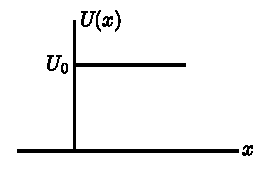
\includegraphics[width=5cm]{fig6.pdf}\\
{\small 图 6}
\end{center}

\begin{center}
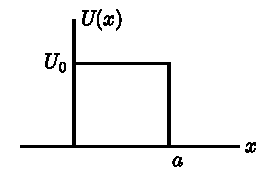
\includegraphics[width=5cm]{fig7.pdf}\\
{\small 图 7}
\end{center}

解：令 $E>U_0$，并设入射粒子自左向右运动.则在不同区域内的波函数表式为
\begin{equation*}
\begin{aligned}
  &x<0\ \text{处},\qquad
  \psi=\mathrm{e}^{\mathrm{i}k_1x}+A\,\mathrm{e}^{-\mathrm{i}k_1x},\\
  &0<x<a\ \text{处},\qquad
  \psi=B\,\mathrm{e}^{\mathrm{i}k_2x}+B'\mathrm{e}^{-\mathrm{i}k_2x},\\
  &x>a\ \text{处},\qquad
  \psi=C\,\mathrm{e}^{\mathrm{i}k_1x}
\end{aligned}
\end{equation*}
（在 $x>a$ 一边只能有沿 $x$ 正方向行进的透射波）.$A,B,B'$ 和 $C$ 等常数可以由 $x=0$，$x=a$ 两处的 $\psi$ 及 $\mathrm{d}\psi/\mathrm{d}x$ 的连续性条件确定.透射系数为
$D=k_1|C|^2/k_1=|C|^2$.由此算得
\begin{equation*}
  D=\frac{4k_1^2 k_2^2}
  {\left(k_1^2-k_2^2\right)^2\sin^2 ak_2+4k_1^2 k_2^2}.
\end{equation*}
$E<U_0$ 时，$k_2$ 是一个纯虚量；上式中的 $k_2$ 可以用 $\mathrm{i}\kappa_2$ 代替，而
$\hbar\kappa_2=\sqrt{2m\left(U_0-E\right)}$，即得相应的 $D$ 式：
\begin{equation*}
  D=\frac{4k_1^2\kappa_2^2}
  {\left(k_1^2+\kappa_2^2\right)^2\sinh^2 a\kappa_2+4k_1^2\kappa_2^2},
\end{equation*}

\noindent{\heiti 习题 3}\quad 求粒子对势壁为
$U(x)=U_0/\left(1+\mathrm{e}^{-\alpha x}\right)$（图 5）的反射系数；该粒子的能量 $E>U_0$.

解：薛定谔方程为
\begin{equation*}
  \frac{\mathrm{d}^2\psi}{\mathrm{d}x^2}
  +\frac{2m}{\hbar^2}
  \left(E-\frac{U_0}{1+\mathrm{e}^{-\alpha x}}\right)\psi=0.
\end{equation*}
我们需要求这样的解，这解当 $x\to+\infty$ 时具有下列形式：
\begin{equation*}
  \psi=\text{常数}\times\mathrm{e}^{\mathrm{i}k_2 x}.
\end{equation*}
引入一新变量
\begin{equation*}
  \xi=-\mathrm{e}^{-\alpha x}
\end{equation*}
（所取之值可从 $-\infty$ 到 0），把该解写成下列形式：
\begin{equation*}
  \psi=\xi^{-\mathrm{i}k_2/\alpha}\,w(\xi),
\end{equation*}
其中的 $w(\xi)$ 当 $\xi\to 0$（即 $x\to\infty$）时应趋于一个常数.结果 $w(\xi)$ 满足下列超几何方程：
\begin{equation*}
  \xi\left(1-\xi\right)w''
  +\left(1-2\mathrm{i}k_2/\alpha\right)\left(1-\xi\right)w'
  +\left(k_2^2-k_1^2\right)w/\alpha^2=0,
\end{equation*}
其解为下列超几何函数：
\begin{equation*}
  w=F\left(\mathrm{i}\,\frac{k_1-k_2}{\alpha},
  -\mathrm{i}\,\frac{k_1+k_2}{\alpha},
  -\frac{2\mathrm{i}}{\alpha}k_2+1,\ \xi\right)
\end{equation*}
（我们略去了一个常因子）.$\xi\to 0$ 时这个函数趋向 1，即已满足所加条件.

$\xi\to-\infty$（即 $x\to-\infty$）时 $\psi$ 函数的渐近式为\footnote{见 (e.6) 式，把该式中的两个 $1/z$ 的超几何函数都改成 1，也就是说，我们只取每项展式中的第一项.}
\begin{equation*}
\begin{aligned}
  \psi&\approx\xi^{-\mathrm{i}k_2/\alpha}
  \left[C_1\left(-\xi\right)^{\mathrm{i}(k_2-k_1)/\alpha}
  +C_2\left(-\xi\right)^{\mathrm{i}(k_1+k_2)/\alpha}\right]=\\
  &=\left(-1\right)^{-\mathrm{i}k_2/\alpha}
  \left[C_1\,\mathrm{e}^{\mathrm{i}k_1 x}
  +C_2\,\mathrm{e}^{-\mathrm{i}k_1 x}\right],
\end{aligned}
\end{equation*}
其中
\begin{equation*}
  C_1=\frac{\Gamma\left(-2\mathrm{i}k_1/\alpha\right)
  \Gamma\left(-2\mathrm{i}k_2/\alpha+1\right)}
  {\Gamma\left(-\mathrm{i}\left(k_1+k_2\right)/\alpha\right)
  \Gamma\left(-\mathrm{i}\left(k_1+k_2\right)/\alpha+1\right)},
\end{equation*}
\begin{equation*}
  C_2=\frac{\Gamma\left(2\mathrm{i}k_1/\alpha\right)
  \Gamma\left(-2\mathrm{i}k_2/\alpha+1\right)}
  {\Gamma\left(\mathrm{i}\left(k_1-k_2\right)/\alpha\right)
  \Gamma\left(\mathrm{i}\left(k_1-k_2\right)/\alpha+1\right)}.
\end{equation*}
所求的反射系数为 $R=|C_2/C_1|^2$；计算时可用下列熟知公式：
\begin{equation*}
  \Gamma(x)\Gamma(1-x)=\pi/\sin\pi x,
\end{equation*}
我们得
\begin{equation*}
  R=\left(\frac{\sinh\left[\pi\left(k_1-k_2\right)/\alpha\right]}
  {\sinh\left[\pi\left(k_1+k_2\right)/\alpha\right]}\right)^2.
\end{equation*}
$E=U_0$（$k_2=0$）时 $R$ 变成 1，而当 $E\to\infty$ 时 $R$ 按以下规律趋于零：
\begin{equation*}
  R=\left(\frac{\pi U_0}{\alpha\hbar}\right)^2
  \frac{2m}{E}\,
  \mathrm{e}^{-\frac{4\pi}{\alpha\hbar}\sqrt{2mE}}
\end{equation*}
经典力学极限情形时 $R$ 果真变成零.

\noindent{\heiti 习题 4}\quad 求粒子穿过下列势垒的透射系数（见图 8）：
\begin{equation*}
  U(x)=U_0/\cosh^2\alpha x,
\end{equation*}
该粒子的能量 $E<U_0$.

\begin{center}
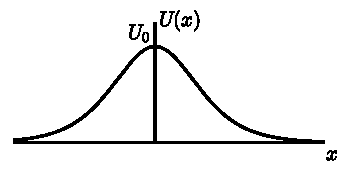
\includegraphics[width=6cm]{fig8.pdf}\\
{\small 图 8}
\end{center}

解：薛定谔方程和§23题 5 的相同，只要把该题中 $U_0$ 的符号更改一下，并把 $E$ 看作正量就可以了.类似的计算给出解
\begin{equation*}
  \psi=\left(1-\xi^2\right)^{-\frac{\mathrm{i}k}{2\alpha}}
  F\left(-\frac{\mathrm{i}k}{\alpha}-s,\,
  -\frac{\mathrm{i}k}{\alpha}+s+1,\,
  -\frac{\mathrm{i}k}{\alpha}+1,\,
  \frac{1-\xi}{2}\right),
\end{equation*}
其中的
\begin{equation*}
  \xi=\tanh\alpha x,
  \qquad
  k=\frac{1}{\hbar}\sqrt{2mE},
\end{equation*}
\begin{equation*}
  s=\frac{1}{2}\left(-1+\sqrt{1-\frac{8mU_0}{\alpha^2\hbar^2}}\ \right).
\end{equation*}
这个解已经满足这样的条件，使得 $x\to\infty$ 即
$\xi\to 1$，$\left(1-\xi\right)\approx 2\,\mathrm{e}^{-2\alpha x}$
时 $\psi$ 中只含透射波（$\sim\mathrm{e}^{\mathrm{i}kx}$）.应用超几何函数变换式 (e.7)，这个波函数当 $x\to-\infty$（$\xi\to-1$）时的渐近式为
\begin{equation*}
  \psi\sim\mathrm{e}^{-\mathrm{i}kx}\,
  \frac{\Gamma\left(\mathrm{i}\frac{k}{\alpha}\right)
  \Gamma\left(1-\frac{\mathrm{i}k}{\alpha}\right)}
  {\Gamma(-s)\Gamma(1+s)}
  +\mathrm{e}^{\mathrm{i}kx}\,
  \frac{\Gamma\left(-\frac{\mathrm{i}k}{\alpha}\right)
  \Gamma\left(1-\frac{\mathrm{i}k}{\alpha}\right)}
  {\Gamma\left(-\frac{\mathrm{i}k}{\alpha}-s\right)
  \Gamma\left(-\frac{\mathrm{i}k}{\alpha}+s+1\right)}.
\end{equation*}
算出上式中两个系数的模量平方比，可得下列形式的透射系数 $D=1-R$
\begin{equation*}
  \frac{8mU_0}{\hbar^2\alpha^2}<1\ \text{时},
  \quad
  D=\frac{\sinh^2\dfrac{\pi k}{\alpha}}
  {\sinh^2\dfrac{\pi k}{\alpha}
  +\cos^2\left(\dfrac{\pi}{2}
  \sqrt{1-\dfrac{8mU_0}{\hbar^2\alpha^2}}\right)};
\end{equation*}
\begin{equation*}
  \frac{8mU_0}{\hbar^2\alpha^2}>1\ \text{时},
  \quad
  D=\frac{\sinh^2\dfrac{\pi k}{\alpha}}
  {\sinh^2\dfrac{\pi k}{\alpha}
  +\cosh^2\left(\dfrac{\pi}{2}
  \sqrt{\dfrac{8mU_0}{\hbar^2\alpha^2}-1}\right)}.
\end{equation*}
第一式对 $U_0<0$ 的情形也适用，此时粒子不是越过势垒而是越过势阱.有趣的是，当
$1+\left(8m|U_0|/\hbar^2\alpha^2\right)=\left(2n+1\right)^2$ 时，$D=1$，也就是说，当阱深 $|U_0|$ 具有适当数值时，在势阱上越过的粒子没有反射.这个结果还可从 (2) 式看出，当 $s$ 为正整数时，该式中的 $\mathrm{e}^{-\mathrm{i}kx}$ 项不再存在.

\noindent{\heiti 习题 5}\quad 设势能 $U(x)$ 当 $|x|\gg a$ 时迅速减小，$a$ 是描写相互作用区域的一个特征尺度，求当 $E\to 0$ 时透射系数趋于零的规律.

解：在距离满足 $k|x|\ll 1$ 的区域，可将薛定谔方程中的能量 $E$ 略去，如果同时 $|x|\gg a$，则连势能也可略去，这时薛定谔方程成为
\begin{equation*}
  -\frac{\hbar^2}{2m}\frac{\mathrm{d}^2\psi}{\mathrm{d}x^2}=0
\end{equation*}
它的解可以写成
\begin{equation*}
\begin{aligned}
  &x<0\ \text{时},\qquad \psi=a_1+b_1 x\\
  &x>0\ \text{时},\qquad \psi=a_2+b_2 x
\end{aligned}
\end{equation*}
在距离为 $x\sim a$ 处解此方程可得出 $a_1 b_1$ 和 $a_2 b_2$ 的关系，这个关系是线性的，并具有下列形式
\begin{equation*}
  a_1=\rho a_2+\mu b_2,
  \qquad
  b_1=\nu a_2+\tau b_2
\end{equation*}
系数 $\rho,\mu,\nu$ 和 $\tau$ 都是实的，并且与能量无关，因为薛定谔方程中已无能量.\footnote{由于概率流是常数，这四个系数满足下列关系：$\rho\tau-\mu\nu=1$.}(1) 式的解应该与函数 (25.1)，(25.2) 按 $x$ 的幂展开式的前两项相一致，即
\begin{equation*}
  a_1=1+B,\qquad
  b_1=\mathrm{i}k\left(1-B\right),\qquad
  a_2=A,\qquad
  b_2=\mathrm{i}k A
\end{equation*}
将这些关系代入 (2) 式，并当 $k$ 小时解出 $A$，得
\begin{equation*}
  A\approx 2\mathrm{i}k/\nu
\end{equation*}
由此得
\begin{equation*}
  D\approx\frac{4k^2}{\nu^2}\sim E
\end{equation*}
于是得，透射系数与粒子的能量成正比地趋于零.在上面例题 2 和例题 4 的例子中，这个一般的规律显然是满足的.

\end{xiti}
